% ------------------------------------------
%  MASTER THESIS DISSERTATION
% ------------------------------------------
% Author: Carlos Silva
%
% Advisor: António Manuel Raminhos Cordeiro Grilo
% Advisor: Naercio David Pedro Magaia
%
% ------------------------------------------
\documentclass[10pt,openright,a4paper]{report}
\usepackage[utf8]{inputenc}

% Set document margins to 1in in all sides
\usepackage[margin=2.5cm, top=2.5cm, bottom=2.5cm]{geometry}
% Line spacing package
\usepackage{graphicx, helvet, hyperref, setspace}
\usepackage[portuguese,english]{babel}
\usepackage[acronym, toc]{glossaries}

% Built the glossary when the main file is built.
\makeglossaries
% Set main font to Arial
\renewcommand{\familydefault}{\sfdefault}
% Define keywords macro
\providecommand{\keywords}[1]{\textbf{Keywords:} #1}
% Define the NewPage macro
\newcommand*\NewPage{\newpage\null\thispagestyle{empty}\cleardoublepage}
% Abstract-en page numbering
%\newcommand {\abstractEnglishPageNumber} {\thispagestyle{plain}\setcounter{page}{\abstractEnglishPage}}
% Abstract-pt page numbering
%\newcommand {\abstractPortuguesePageNumber} {\thispagestyle{plain}\setcounter{page}{\abstractPortuguesePage}}
% Section numbering depth
\setcounter{secnumdepth}{2}
% Table of contents depth
\setcounter{tocdepth}{3}
% Set line spacing to 1.5cm
\onehalfspacing
% Page numbering
%\pagestyle{plain}

% Glossary Definition
\newglossaryentry{MSc}{name={MSc}, description={Masters degree in the area of Science.}}
\newglossaryentry{maths}
{
    name=mathematics,
    description={Mathematics is what mathematicians do}
}

% Acronym-Definition
\newacronym{IST}{IST}{Instituto Superior T\'ecnico}
\newacronym{UE}{UE}{User Equipment}
\newacronym{IoT}{IoT}{Internet of Things}
\newacronym{CC}{CC}{Cloud Computing}
\newacronym{QoS}{QoS}{Quality-of-Service}
\newacronym{MEC}{MEC}{Mobile Edge Computing}
\newacronym{ETSI}{ETSI}{European Telecommunications  Standards  Institute}
\newacronym{MDP}{MDP}{Markov Decision Process}
\newacronym{DNN}{DNN}{Deep Neural Networks}
\newacronym{RL}{RL}{Reinforcement Learning}
\newacronym{DRL}{DRL}{Deep Reinforcement Learning}
\newacronym{FC}{FC}{Fog Computing}
\newacronym{SDN}{SDN}{Software Defined Network}
\newacronym{ISG}{ISG}{Industry Specification Group}
\newacronym{RAN}{RAN}{Radio Access Network}
\newacronym{SCC}{SCC}{Small Cell Cloud}
\newacronym{SCM}{SCM}{Small Cell Manager}
\newacronym{MMC}{MMC}{Mobile Micro Cloud}
\newacronym{MobiScud}{MobiScud}{Fast  Moving  Personal  Cloud}
\newacronym{MC}{MC}{MobiScud Control}
\newacronym{FMC}{FMC}{Follow  Me  Cloud}
\newacronym{SCeNBs}{SCeNBs}{Small Cells}
\newacronym{eNB}{eNB}{Wireless Base Station}
\newacronym{CN}{CN}{Core Network}
\newacronym{NFV}{NFV}{Network Function Virtualization}
\newacronym{POMDP}{POMDP}{Partially  Observable  Markov  Decision  Process}
\newacronym{ANNs}{ANNs}{Artificial Neural Networks}
\newacronym{DQN}{DQN}{Deep Q-Network}
\newacronym{CNNs}{CNNs}{Convolutional Neural Networks}
\newacronym{RNNs}{RNNs}{Recurrent Neural Networks}
\newacronym{DDQN}{DDQN}{Double Deep Q-Network}
\newacronym{TD}{TD}{Temporal Difference}
\newacronym{Dueling DQN}{Dueling DQN}{Dueling Deep Q-Network}
\newacronym{A3C}{A3C}{Asynchronous Advantage Actor-Critic}
\newacronym{A2C}{A2C}{Advantage Actor-Critic}
\newacronym{AGA}{AGA}{Adaptive Genetic Algorithm}
\newacronym{IaaS}{IaaS}{Infrastructure as a Service}
\newacronym{VMs}{VMs}{Virtual Machines}
\newacronym{GPU}{GPU}{Graphics Processing Unit}
\newacronym{CPU}{CPU}{Central Processing Unit}
\newacronym{DRQN}{DRQN}{Deep Recurrent Q-Network}

\usepackage{hyperref}
\hypersetup{
    colorlinks=true,
    linkcolor=black,
    filecolor=magenta,      
    urlcolor=cyan,
    citecolor=blue,
}


\newcommand{\cmmnt}[1]{\ignorespaces}

\renewcommand{\baselinestretch}{1.5}

\usepackage{indentfirst}
\usepackage{float}
\usepackage{amsfonts}
\usepackage{amssymb}
\usepackage{amsmath}
\usepackage{optidef}
\usepackage{algorithm}
\begin{document}

\pagenumbering{gobble}% Remove page numbers (and reset to 1)
\clearpage
%\thispagestyle{empty}
%!TEX root = ./dissertation.tex

% Dissertation basic information
\newcommand {\Title} {Task offloading optimization in Mobile Edge Computing (MEC) based on Artificial Intelligence (AI)}
%\newcommand {\Subtitle} {My Subtitle}
\newcommand {\StudentName} {Carlos Alexandre Marques Alves da Silva}
%\newcommand {\DegreeName} {Mestrado Integrado de Engenharia Eletroténica e de Computadores}
\newcommand {\DegreeName} {Electrical and Computer Engineering}
\newcommand {\Supervisors} {{\large Prof. Pedro Tiago Martins Batista},{\large Prof. Pedro Tiago Martins Batista}}

% Include or not include acknowledgments
%\def \includeAcknowledgments{1}

% Include or not include glossary
%\def \includeGlossary{0}

% Examination Committee
\newcommand {\Chairperson} {{\large Prof./Dr.}}
\newcommand {\Advisor} {{\large Prof./Dr.}}
\newcommand {\CommitteeMembers} {
{\large Prof./Dr.}\\
{\large Prof./Dr.}
}

% Date
\newcommand {\Month} {January}
\newcommand {\Year} {2020}

% Acknowledgments page number
\def \acknowledgmentsPage{1}

% Abstract-en page numbering
\def \abstractEnglishPage{3}

% Abstract-pt page number
\def \abstractPortuguesePage{5}

% You can define your own variables here

%!TEX root = ./dissertation.tex

% ---------------------------------------------------------
%   MASTER THESIS DISSERTATION COVER
% ---------------------------------------------------------
\begin{titlepage}
% ---------------------------------------------------------
%  INSTITUTION LOGO
% ---------------------------------------------------------

\includegraphics[width=5cm]{images/ist_logo}~\\[2.0cm]
\begin{center}
% ---------------------------------------------------------
%  MASTER THESIS DISSERTATION TITLE
% ---------------------------------------------------------
{\LARGE \textbf{\Title}}\\[2.5cm]
% ---------------------------------------------------------
%  MASTER THESIS DISSERTATION SUBTITLE
% ---------------------------------------------------------
%{\Large \Subtitle}\\[1.0cm]
% ---------------------------------------------------------
%  AUTHOR NAME (FULL)
% ---------------------------------------------------------
{\Large \textbf{\StudentName}}\\[2.0cm]
% ---------------------------------------------------------
%  DISSERTATION DEGREE
% -----------------------------------------------------------------
{\large Thesis to obtain the Master of Science Degree in}\\[0.5cm]
% -----------------------------------------------------------------
%  COURSE NAME
% -----------------------------------------------------------------
{\LARGE \textbf{\DegreeName}}\\[1.5cm]

% -----------------------------------------------------------------
%  ADVISORS NAME
% ---------------------------------------------------------
%\begin{minipage}[t]{.5\textwidth}
  %\begin{flushright}
  %  {\large Supervisor:\:}
 % \end{flushright}
%\end{minipage}%
%\begin{minipage}[t]{.5\textwidth}
  %\begin{flushleft}
  %  {\Supervisors}
 % \end{flushleft}
%\end{minipage}\\[5.0cm]
{\large Supervisor: \ Prof. António Manuel Raminhos Cordeiro Grilo}\\
{\large Co-Supervisor: \ Prof. Naercio David Pedro Magaia}\\[2cm]
% ---------------------------------------------------------
%  JURI NAMES:
%  - PRESIDENT
%  - ADVISOR
%  - VOGALS
% ---------------------------------------------------------
{\Large \textbf{Examination Committee}}\\[1cm]
%\begin{minipage}[t]{.5\textwidth}
%  \begin{flushright}
%    {\large Chairperson:\:}\\
%    {\large Advisor:\:}\\
%    {\large Members of the %Committee:\:}
%  \end{flushright}
%\end{minipage}%
%\begin{minipage}[t]{.5\textwidth}
%  \begin{flushleft}
%    {\Chairperson}\\
%    {\Advisor}\\
%    {\CommitteeMembers}
%  \end{flushleft}
%\end{minipage}\\[1.0cm]
{\large Chairperson: \ Prof. José Eduardo Charters Ribeiro da Cunha Sanguino}\\
{\large Supervisor: \ Prof. António Manuel Raminhos Cordeiro Grilo}\\
{\large Co-Supervisor: \ Prof. Naercio David Pedro Magaia}\\
{\large Member of the Committee: \ Prof. Paolo Romano}\\[2cm]


% ---------------------------------------------------------
%  DATE (MONTH AND YEAR)
% ---------------------------------------------------------
{\Large \textbf{June\:2022}}\\
\end{center}
\end{titlepage}
%\NewPage

\setcounter{page}{1} \pagenumbering{roman}

\section*{Abstract}

% Add entry in the table of contents as section
\addcontentsline{toc}{section}{Abstract}

\noindent The \acrfull{CC} paradigm has risen in recent years as a solution to a need for computation and battery constrained \acrfull{UE} to run increasingly intensive computation tasks. Given its seemingly infinite amount of resources and pay as you go nature this paradigm has brought several advantages: 1) Extended battery life of \acrfull{UE}s by offloading computation; 2) Enables new types of applications intractable with \acrfull{UE}'s computation capabilities; 3) In an ever more data focused world it allows for unlimited storage capacity. Nevertheless, given the centralized nature of the \acrshort{CC} paradigm this option introduces significant network congestion problems and unpredictable communication delay not suitable for real-time applications. To cope with these problems the \acrfull{MEC} concept has been introduced, which proposes to bring computation resources closer to the edge of the mobile networks in a distributed way. However, given that these edge computation resources are limited, this paradigm comes with its set of challenges that need to be solved in order to make it viable. In this work a review of several \acrshort{MEC} architectures is made. Subsequently the state of the art on \acrfull{DRL} and their application to the \acrshort{MEC} challenges is explored. This work proposes to innovate by presenting a network management agent capable of making offloading decisions from an heterogeneous network of \acrshort{UE}s to an  heterogeneous network of \acrshort{MEC} servers. This agent represents an orchestrator of a group of 5G \acrfull{SCeNBs}, enhanced with computation and storage capabilities. In order to solve this high complexity problem, an \acrfull{A2C} agent is implemented and tested against several baselines. The proposed solution is shown to beat the baselines by making intelligent decisions taking into
account computation, battery, delay and communication constraints ignored by the baselines. The solution is also shown to be scalable, data efficient, robust, stable and adjustable to address not only overall system performance but to take into account the worst case scenario.

\vfill

\textbf{\Large Keywords:} Mobile Edge Computing, Computation Offloading, Energy and Performance Optimization, Delay Sensitivity, Deep Reinforcement Learning, Cloud Computing


\clearpage
\section*{Resumo}

% Add entry in the table of contents as section
\addcontentsline{toc}{section}{Resumo}

\noindent Nos últimos anos o paradigma de Computação em Nuvem (\acrshort{CC}) tem vindo a crescer como uma solução para a necessidade de correr computações cada vez mais complexas em Equipamentos de Utilizador (\acrshort{UE}) limitados a nível de computação e bateria. Devido à quantidade aparentemente infinita de recursos computacionais e sua natureza de pagamento conforme o uso, este paradigma trouxe várias vantagens: 1) Ao transferir computação poupa a bateria dos \acrshort{UE}s; 2) Permite novas aplicações complexas não executáveis com os recursos dos \acrshort{UE}s; 3) Num mundo cada vez mais focado em dados, permite o armazenamento ilimitado dos mesmos. No entanto, dada a natureza centralizada do paradigma \acrshort{CC} existem problemas de congestionamento de rede significativos e atrasos de comunicação imprevisíveis e inadequados para aplicações em tempo real. O conceito de \emph{Mobile Edge Computing} (\acrshort{MEC}) surgiu para lidar com estes problemas e tem como ideia principal aproximar os recursos de computação de forma distribuída ao limite das redes móveis. Por vez, como esses recursos de computação são limitados, este novo paradigma apresenta um conjunto de desafios que precisam de ser resolvidos de maneira a torná-lo viável. Neste trabalho é feita uma revisão de várias arquitecturas de \acrshort{MEC}. Subsequentemente, o estado da arte em Aprendizagem por Reforço Profunda (\acrshort{DRL}) e a sua aplicação aos desafios do paradigma \acrshort{MEC} são explorados. Este trabalho propõe então inovar apresentando um agente de gestão de rede capaz de tomar decisões de offloading de uma rede heterogênea de \acrshort{UE}s para uma rede heterogênea de servidores \acrshort{MEC}. Este agente representa um orquestrador de um grupo de \emph{Small Cells} (\acrshort{SCeNBs}) de 5G, dotados de capacidades de computação e armazenamento. De maneira a resolver este problema de elevada complexidade foi implementado um agente \emph{Advantage Action-Critic} (\acrshort{A2C}) e este foi testado contra um grupo de algoritmos base. A solução proposta demonstra capacidade de bater os algoritmos base tomando decisões inteligentes que têm em conta limitações de computação, bateria, atraso e comunicação, ignoradas pelos algoritmos base. É também demonstrado que a solução é escalável, eficiente de um ponto de vista de dados, robusta, estável e ajustável para ter em consideração não só o custo do sistema como um todo mas ter também em conta o pior caso do mesmo. 

\vfill

\textbf{\Large Palavras Chave:} \emph{Mobile Edge Computing}, \emph{Offloading} Computacional, Optimização Energética e de Execução, Restrições de Latência, Aprendizagem por Reforço Profunda, Computação em Nuvem


%\clearpage

% Table of contents
\tableofcontents
\printglossaries
\clearpage
% A new page is necessary only if table of contents has an even number of pages


\pagenumbering{arabic}


\chapter{Introduction}
\label{chapter:introduction}
\setcounter{page}{1}
\section{Context}
\noindent There has been a continuous exponential increase in the number of \acrfull{UE}, such as smartphones, laptops and \acrfull{IoT} devices. Their need to run ever more complex applications, given their energy and computation constrained environment, has led to the rise of \acrfull{CC} as an alternative to offload computation and storage needs. In the \acrshort{CC} paradigm, computation resources are located in centralized data centers that can be considered infinite. This paradigm brings several advantages \cite{SHAKARAMI2020107496}: 
\begin{enumerate}
    \item By offloading computation, it extends the battery life of \acrshort{UE}; 
    \item Enables computationally complex applications intractable with \acrshort{UE} computation capabilities;
    \item Provides seemingly unlimited storage capacity.
\end{enumerate}
However, there are also shortcomings. The two main problems introduced by this paradigm are: 
\begin{enumerate}
    \item The distance from \acrshort{UE}s to these servers introduces an unpredictable communication latency that makes some delay-constrained applications unviable;
    \item  This increase in \acrshort{UE}s and their communication needs with \acrshort{CC} servers leads to ever more congested network links decreasing \acrfull{QoS} for everyone in the network.
\end{enumerate}

\par
These shortcomings gave rise to a new emerging concept known as \acrfull{MEC}. The main idea of \acrshort{MEC} is to bring computation resources closer to the edge of the mobile network enabling offloading of complex computation tasks with strict delay requirements. As defined by the \acrfull{ETSI} in \cite{MECspec}, this can be achieved by allocating computing nodes at the network's edge in a fully distributed manner to reduce communication overhead and execution delay for \acrshort{UE}s.

\clearpage

\section{Motivation}
\noindent Edge computing nodes come with limited radio, storage and computational resources, which raise three main challenges \cite{SHAKARAMI2020107496}:
\begin{itemize}
    \item The \textbf{decision of which computing tasks} are profitable for the \acrshort{UE} to offload to the \acrshort{MEC} servers in terms of energy consumption and execution delay.
    \item How to efficiently \textbf{allocate the limited computation resources} within the \acrshort{MEC} servers in order to minimize response delay and load balance the computing resources and communication links.
    \item \textbf{Mobility management} to guarantee \acrshort{MEC} service continuity and efficiency for \acrshort{UE}s roaming the network.
\end{itemize}

Given the heterogeneous and stochastic nature of network topologies, traditional optimization techniques lack the scalability and adaptability to deal with unknown network conditions. Recent breakthroughs in machine learning algorithms, showcasing their ability to solve and adapt to complex problems previously thought impossible to be solved by a computer, led many researchers to explore applying these methods to the \acrshort{MEC} challenges.
\par
The problem of making offloading and resource allocation decisions in \acrshort{MEC} can be simulated and performance benchmarks are easily defined. This makes their definition as a \acrfull{MDP} straightforward and allows the use of promising algorithms, like \acrfull{DNN} trained using \acrfull{RL} or \acrfull{DRL} algorithms for short. 

\section{Objectives}
\noindent The main goal of this work is to expand the research efforts in \acrshort{MEC} with the development of a network management agent capable of making offloading decisions from a heterogeneous network of \acrshort{UE}s to a heterogeneous network of \acrshort{MEC} servers. These decisions should take into account the battery, computation and communication constrains of each \acrshort{UE} and \acrshort{MEC} server.
\par
To achieve this goal multiple related works were studied in order to develop a realistic network simulation environment, understand the state-of-the-art in \acrshort{DRL} algorithms and their application to the \acrshort{MEC} challenges.

\section{Contributions}
\noindent The main contributions of this work are:
\begin{itemize}
    \item The release of an open-source realistic network simulation environment as an OpenAI Gym, \cite{opengym}, enviroment. Allowing for easy experimentation with different \acrshort{DRL} algorithms;
    \item The implementation of an open-source, \acrshort{A2C} agent, capable of making intelligent offloading decisions that take into account battery, computation and communication constraints overperforming the baselines in a heterogeneous network of several \acrshort{UE}s and \acrshort{MEC} servers;
\end{itemize}

The code for the simulator, baselines and agent, as well as environment configurations can be found in the following code repository:
\href{https://github.com/Carlos-Marques/rl-MEC-scheduler}{https://github.com/Carlos-Marques/rl-MEC-scheduler}.

\section{Report outline}
\noindent This document is structured as follows:
\begin{itemize}
    \item Chapter 1 serves as a brief introduction and motivation for the work done in this thesis. In particular, the relevance of \acrshort{MEC} in the current and future technological landscape and its current challenges.
    \item In Chapter 2, first, a review of several \acrshort{MEC} network architectures is made. Then, \acrshort{DRL} concepts  and  algorithms  are  introduced. Finally, related works using \acrshort{DRL} methods to solve challenges in \acrshort{MEC} are explored.
    \item Chapter 3 focuses on defining the problem statement, the proposed solution and the methods and tools.
    \item Chapter 4 serves to showcase baseline algorithms and test the agent's performance in terms of learning capacity, scalability, data efficiency, robustness, stability and adjustability. 
    \item In Chapter 5, first, a summary about this work is made. Then future work is explored.
\end{itemize}







 







\chapter{State of the art}
\label{chap:stateoftheart}
\section{Overview of \acrshort{MEC} architectures} \label{section:MECarch}

\noindent One of the first efforts to bring computation resources closer to the edge was the cloudlet concept presented in \cite{cloudlet}. The main idea behind it was to allocate powerful computers at WiFi hotspots that could sell their \acrfull{IaaS} through the use of \acrfull{VMs}.

Another concept to bring computation closer to \acrshort{UE}s is the idea of an \emph{ad-hoc} cloud like the one presented in \cite{adhoc}. The idea proposes that the computation power of a network of non-exclusive and sporadically available hosts can be harvested and abstracted as a service to which \acrshort{UE}s can offload their computational needs.

In order to standardize and generalize other concepts of edge computing, the OpenFog Consortium proposes a standard \acrfull{FC} architecture \cite{OpenFog}. This architecture presents computation resources as a continuum between the \acrshort{UE}s and the cloud by abstracting edge computing platforms like cloudlets or ad-hoc clouds as fog nodes that make their services available to \acrshort{UE}s. These fog nodes can be organized physically or by a \acrfull{SDN} and share their workload, making offloading decisions on \acrshort{UE} tasks to other fog nodes or \acrshort{CC} centralized data centers whenever needed.

While \acrshort{FC} is defined in \cite{OpenFog} as a system-level horizontal architecture that distributes resources and services of computing, storage, control and networking anywhere along the continuum from a cloud data center down to users. the \acrfull{MEC} concept presented by the \acrfull{ISG} within the \acrfull{ETSI} in \cite{MECspec} is focused on integrating computation resources within the \acrfull{RAN} in very close proximity to mobile subscribers.

As presented in paper \cite{SHAKARAMI2020107496}, several \acrshort{MEC} architectures have been proposed in order to integrate and manage computation resources at the \acrshort{RAN} level, such as \acrfull{SCC} \cite{smallcellcloud}, \acrfull{MMC} \cite{mmcloud}, \acrfull{MobiScud} \cite{MobiScud}, \acrfull{FMC} \cite{fmcloud} and CONCERT \cite{CONCERT}. These architectures differ mainly in terms of distance from \acrshort{UE}s to computation resources and can then be divided into two main types: 1) edge computing at the access node level; 2) distributed data centers. Finally, the CONCERT architecture merges ideas present in \acrshort{SCC} and \acrshort{MMC} with the ideas of \acrshort{MobiScud} and \acrshort{FMC}.

\subsection{Edge computing access nodes}

\noindent The main idea of architectures like \acrfull{SCC} and \acrfull{MMC} is allocating computation resources at the access node level of a mobile network.

The \acrfull{SCC} architecture was first introduced by the European project TROPIC \cite{smallcellcloud} and later expanded by the SESAME project \cite{SESAM}. It proposes that low-powered cellular radio access nodes, i.e. \acrshort{SCeNBs}, be enhanced with computation and storage capabilities. Because of the current popularity of \acrshort{SCeNBs} in 4G networks and their estimated wide adoption as a solution to guarantee the data capacities of 5G networks, this architecture could provide ample computation resources for applications with high latency requirements.

These computation resources at the \acrshort{SCeNBs} would be pooled and presented as a service to \acrshort{UE}'s applications through a management agent. This so-called \acrfull{SCM} could be deployed in a distributed hierarchical manner with a local \acrshort{SCM} managing a cluster of \acrshort{SCeNBs} while being connected to other \acrshort{SCM}s through a remote \acrshort{SCM} located at the \acrshort{CN} of the service provider. The local \acrshort{SCM} would need to be aware of the state of its cluster of \acrshort{SCeNBs} and make offloading decisions on how to distribute work within its cluster. The remote \acrshort{SCM} could help distribute work between local \acrshort{SCM}s by offloading computations to neighboring clusters. This topology can be seen as a \emph{N} to \emph{N} problem where \emph{N} \acrshort{UE}s offload computation to \emph{N} \acrshort{MEC} servers located at the \acrshort{SCeNBs} level.

In the case of the \acrfull{MMC} presented in \cite{mmcloud}, the main idea is to allocate a \acrshort{MEC} server along with the \acrfull{eNB} instead of one at every SCeNB. This topology could then be seen as a \emph{N} to 1 problem where \emph{N} \acrshort{UE}s offload computation to 1 \acrshort{MEC} server located at the \acrshort{eNB} level. These \acrshort{MEC} servers would then be interconnected directly or through backhaul to each other in order to guarantee \acrshort{QoS} in the mobility management of \acrshort{UE}s.

\subsection{Distributed data centers}
\noindent The main idea behind proposed architectures like the \acrfull{MobiScud} \cite{MobiScud} and \acrfull{FMC} \cite{fmcloud} is to integrate cloud services into the mobile networks using data centers closer to the edge of the network.

As presented in \cite{MobiScud}, the \acrfull{MobiScud} architecture makes use of network operator's data centers located within \acrshort{RAN} or close to \acrshort{RAN} instead of allocating computation resources at the access node level like \acrshort{SCC} or \acrshort{MMC} architectures. By using \acrfull{SDN} and \acrfull{NFV} technologies, it proposes to integrate cloud services seamlessly at the mobile network level. This type of architecture introduces the concept of a \acrfull{MC} agent that interfaces with the mobile network, \acrshort{SDN} switches and the cloud operator in order to orchestrate and route data between the various composing operator's clouds in order to maintain \acrshort{QoS} when the \acrshort{UE} moves through the network.

The \acrfull{FMC} architecture proposed in \cite{fmcloud} follows a similar idea to the \acrshort{MobiScud} architecture but instead of using the operator's data centers at the RAN level, it assumes the use of distributed data centers moved farther away into the \acrfull{CN} of the operator.

\subsection{CONCERT architecture}
\noindent As proposed in \cite{CONCERT}, the CONCERT architecture exploits the \acrshort{NFV} and \acrshort{SDN} technologies in order to define a decoupled control/data model.
The data plane is composed by the \acrshort{eNB}, \acrshort{SCeNBs}, \acrshort{SDN} switches and computation resources, being them at the access node level, local data centers or even remote data centers.
The control plane is composed by the management agent, referred to as the conductor, which has access to the network state and manages its resources presenting them as software defined services to \acrshort{UE}'s applications. This type of centralized approach is a clear example of an orchestration approach. As an alternative, a choreography approach is when entities cooperate in a decentralized manner without holding complete knowledge of the network, as is the case of the solution presented in \cite{fogmulti}.

% TODO: add a better transition from MEC achitectures to RL

\section{Reinforcement Learning (RL)} \label{section:RL}
\noindent There are three main machine learning paradigms, supervised learning, unsupervised learning and reinforcement learning. While supervised learning needs a lot of labeled input/output data and unsupervised learning learns patterns from unlabeled data, \acrfull{RL} is used in problems where an agent learns to solve a closed-loop problem by changing its future actions based on a reward resulting from its actions on the environment and its effects on its state.

This paradigm has shown great potential in solving environments that can be simulated and easily benchmarked, which is the reason most research on \acrshort{RL} is made by solving video games, which offer a perfect environment in terms of reproducibility, easy simulation and baked in benchmarks that can be used to compute a reward signal (points, levels, etc.).

\acrshort{RL} tasks are usually modeled as Markov Decision Processes.

\subsection{Markov Decision Process (MDP)}
\noindent The \acrlong{MDP} is a mathematical framework that can be used to model a time-discrete decision process in a stochastic environment as long as it satisfies the Markov property, which states that given the present, the future does not depend on the past.

\acrshort{MDP}s are usually defined by a four-element tuple $<S, A, P, R>$:
\begin{itemize}
    \item $S$ is the state space, which represents the set of all agent and environment states, $s_t \in S$;
    \item $A$ is the action space, which represents the set of all possible agent actions, $a_t \in A$;
    \item $P:S \times A \times S \rightarrow [0, 1]$ is the transition probability distribution $P(s_{t+1}|s_t,a_t)$ of a new state $s_{t+1}$ given that the system is in state $s_t$ and action $a_t$ is chosen;
    \item $R:S\times A \rightarrow \mathbb{R}$, is the reward signal, $r_t$, of the system when action $a_t$ is taken from state $s_t$ to $s_{t+1}$.
\end{itemize}

Many \acrshort{RL} tasks can be approximated as \acrshort{MDP} with careful definition of the state signal, $s_t$, to include past relevant information for the current action decision, $a_t$.

As stated in \cite{RLbook}, given these conditions, the system dynamics can be defined entirely by the current state's probability distribution:
\begin{equation}
p(s', r|s, a) = P(S_t=s', R_t=r|S_{t-1}=s, A_{t-1}=a).
\end{equation}

\acrshort{MDP} assumes full observability of the current environment/agent state. Alternatively, the agent is said to have partial observability when it can only observe part of the entire environment or its observations are corrupted. These types of problems are formulated as \acrfull{POMDP}.

\subsection{Partially Observable Markov Decision Process (POMDP)}
\noindent As a generalization of a \acrshort{MDP}, in a \acrshort{POMDP}, the agent does not have access to the complete state. Instead, a sensor model must be defined on top of the usual \acrshort{MDP} definition. For this reason, an \acrshort{POMDP} is usually defined as a six-element tuple $<S, A, P, R, R, \Omega, O>$ \cite{POMP}, where the new $\Omega$ and $O$ define the sensor model:
\begin{itemize}
    \item $\Omega$ is the set of observations, where $o_t \in \Omega$ is the observation of the agent at time step $t$;
    \item $O$ is the set of conditional probabilities of observation $O(o_{t}|s_{t+1},a_t)$. This means the probability of the observation, $o_t$, given the new state $s_{t+1}$ resulting from the action $a_t$.
\end{itemize}
\subsection{Value function}
\noindent The goal of an \acrshort{RL} agent is to learn a policy, $\pi$, that maximizes the expected cumulative reward:

\begin{equation}
\pi:A \times S \rightarrow [0, 1],
\end{equation}

\begin{equation} \label{policy_func}
\pi(a, s) = P(a_t=a|s_t=s).
\end{equation}

The expected cumulative reward for a given policy starting in state $s_0=s$, can be defined as the value function:

\begin{equation}\label{Vfunction}
V_{\pi}(s)=E[R]=E[\sum\limits_{t=0}^\infty \gamma^t r_t | s_0 = s],
\end{equation}

where the return, $R$, is the sum of future rewards discounted according to the discount-rate, $\gamma \in [0, 1]$:

\begin{equation} \label{return_func}
R = \sum\limits_{t=0}^\infty \gamma^t r_t .
\end{equation}

The discount-rate $\gamma$ is a hyper-parameter that represents how much the agent values future rewards in comparison with current rewards. If $\gamma=0$, then the agent only cares about instant reward. If $\gamma=1$ and the system has no final state, then the problem of calculating the return, $R$, becomes infinite.

The goal can then be defined as finding a policy, $\pi$, that maximizes $V_\pi(s)$:

\begin{equation} \label{maximizes_expected}
V^*(s)=\max\limits_{\pi}V_\pi(s) .
\end{equation}

An action-value function can then be defined as the expected return of taking action $a$, in state $s$, and then following policy $\pi$:

\begin{equation}
Q_\pi(s,a) = E[R|s, a, \pi] .
\end{equation}

Given the optimal policy, $\pi^*$, we can take the optimal action by choosing the action, $a$, with the highest, $Q_{\pi^*}(s,a)$, value. 

Given full knowledge of the \acrshort{MDP}, this problem can be solved using classical dynamic programming techniques like value and policy iteration in which expected values are computed over the whole state-space in order to approximate the optimal action-value function, $Q^*$. These methods have two major problems. First, they assume complete knowledge of the \acrshort{MDP}, wherein most \acrshort{RL} tasks, the transition probability distribution, $P$, and reward signal, $R$, are usually unknown \emph{a priori} and need to be learned from experience. Second, given the brute force nature of these algorithms, they become intractable for higher dimension state-spaces.

One algorithm that tries to learn the action-value function from experience without needing to maintain a model of the environment is the Q-learning algorithm.
\subsection{Q-learning}
\noindent The Q-learning algorithm tries to approximate the action-value function through continued experience on the environment.

\begin{equation}
    Q:S\times A \rightarrow \mathbb{R}
\end{equation}\label{Qval}

This can be done my maintaining a Q-table with a row for each state and a column for each possible action. Each of the cells of the Q-table correspond to the action-value, $Q(s,a)$, and is usually initialized as an arbitrary fixed value. 

At each time step $t$, an action $a_t$, is taken on the state $s$, resulting in a new state $s_{t+1}$, and in a reward $r_t$. Given these values, the Q-table is updated according to: 

\begin{equation}
    Q_{t+1}(s_t, a_t) \leftarrow Q_{t}(s_t, a_t) + \alpha \cdot (r_t + \gamma \cdot \max\limits_{a_{t+1}}Q_t(s_{t+1}, a_{t+1}) - Q_t(s_t, a_t)) ,
\end{equation}

where $\alpha \in [0, 1]$ is the learning rate, which is a hyper-parameter that determines how much new information should affect the current belief.

Unlike Monte Carlo methods, which separate sampling from the environment from updating the policy based on the results, Q-learning is a \acrfull{TD} method, which means that as it follows the policy to explore the environment, it also updates the action-value estimations in an online fashion.

The simple Q-table approach to Q-learning has a glaring issue with higher dimension state and action spaces because it maintains a $Q$ value for each state and action combination. An alternative to the Q-table is using the capabilities of information encoding of \acrfull{ANNs} to approximate the action-value function.

\subsection{Deep Q-Network (DQN)}
\noindent \acrshort{DQN} was proposed in \cite{DQN} as a non-linear approximator of the action-value function in Q-learning. It proposes to solve the memory issues and the time required to explore each state in Q-tables and other function approximation methods. Due to the capabilities of \acrshort{ANNs} to encode information and generalize lessons from experiences to unseen inputs, \acrshort{DQN}s are able to solve problems with state and action spaces of higher dimensions, like playing video games from pixels and game scores, while requiring less memory and computation than other methods.

The main idea is to substitute the Q-table or other function approximation methods with \acrshort{ANNs} composed of multiple layers of neuron-inspired nodes with different activation functions. A diagram comparing the Q-table to the \acrshort{DQN} architecture can be seen in Figure \ref{dqnvsqtable}. These \acrshort{ANNs} have been shown to be able to solve complex representation problems by maintaining simpler internal representations. A simple model of this neuron behavior can be defined as:

\begin{equation}
    y_j = f(\sum w_{ij}x_i + b) ,
\end{equation}

where $y_j$ is the output resulting from the application of a non-linear activation function, $f(.)$, to the sum of each input $x_i$ multiplied by the learned weights $w_{ij}$ offset by a bias value, $b$.

Based on the internal structure and composition of each layer, there are many types of \acrshort{ANNs}. One important type are the \acrfull{CNNs}, which maintain convolutional layers that are specially equipped for tasks where spatially closer inputs can be assumed to be somehow related. These visual cortex inspired processes makes them very good at processing high dimension input images. 

Another important class of \acrshort{ANNs} are the \acrfull{RNNs}, which maintain an internal state memory in some neurons, making them good candidates in problems with correlated sequences of inputs.

\begin{figure}[h]
  \centering
  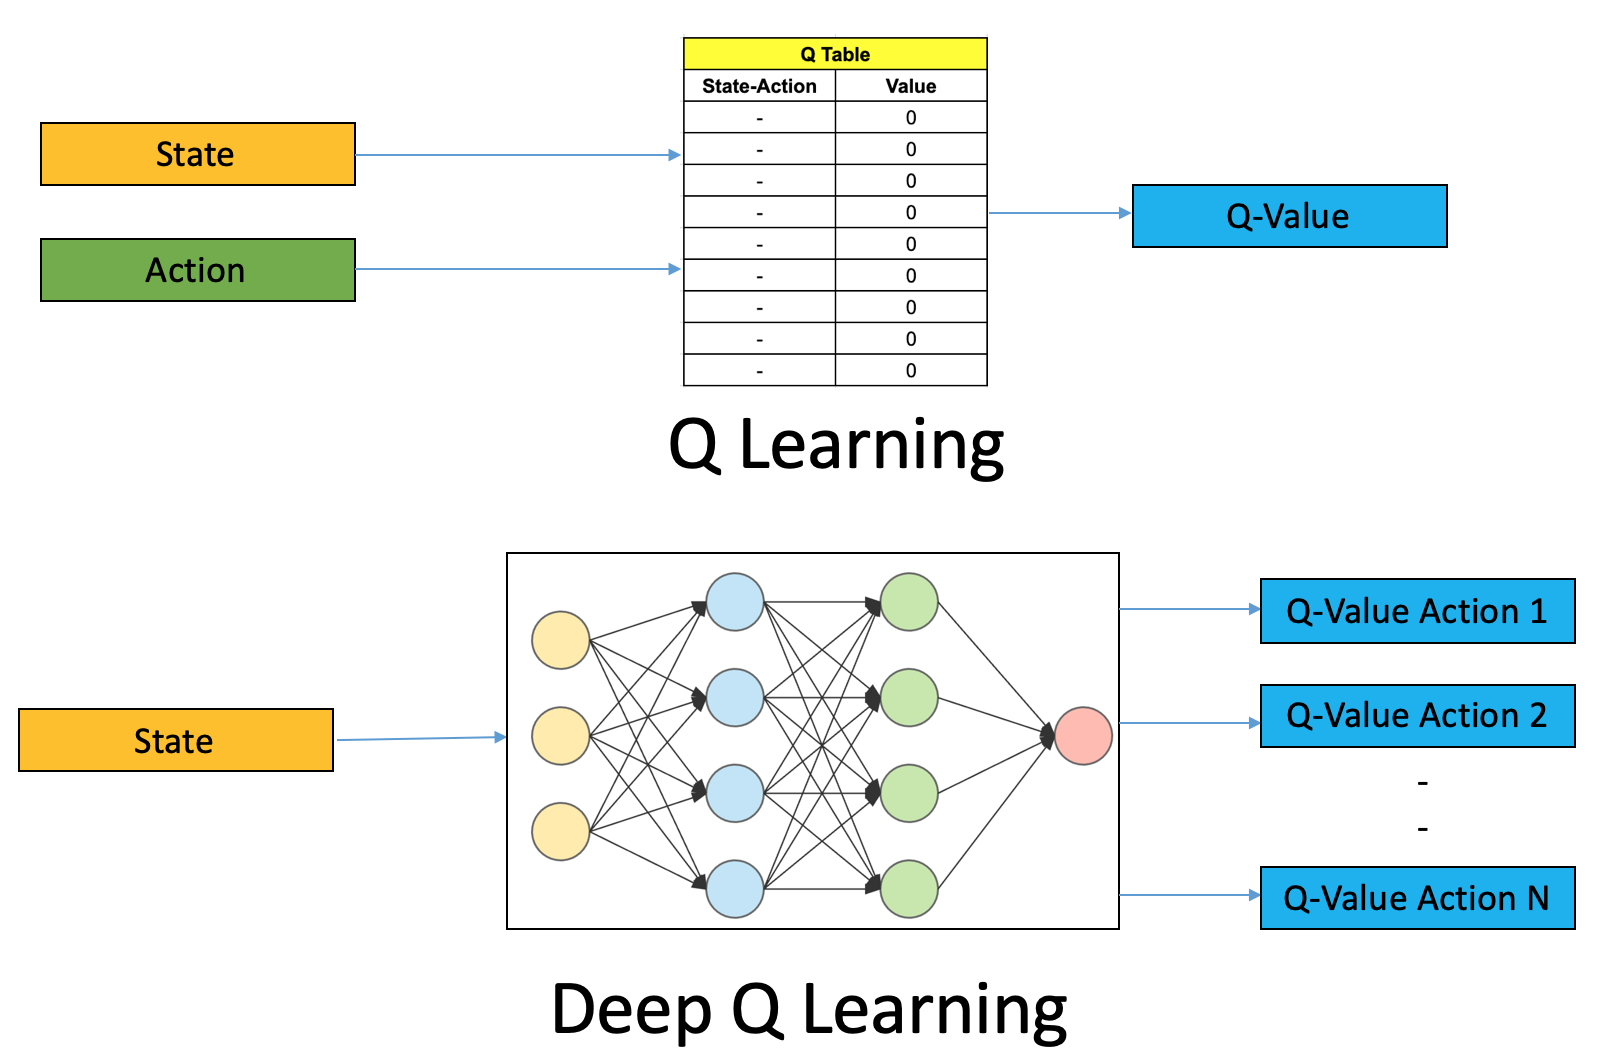
\includegraphics[width=\textwidth]{images/DQN.png}
  \caption{Deep Q Learning architecture comparison with Q-table from \cite{dqnimage}.} \label{dqnvsqtable}
\end{figure}

The proposed ANN in \cite{DQN} is a CNN that can be defined by its weights, $\theta_i$, at each iteration. In order to solve the instability and divergence issues found when using a non-linear function approximator of the action-value function, two methods are proposed. Because these issues arise from the correlations present in the sequence of observations, the paper first proposes a biologically inspired mechanism termed experience replay that collects samples from interaction with the environment in a replay buffer, $U(D)$, and samples randomly from it for training. The second method is an iterative update policy that only adjusts the target weights, $\theta_i^-$, to the new computed weights, $\theta_i$, every $C$ steps.

Since we are dealing with reinforcement learning, the loss function of these \acrshort{ANNs} can not be derived directly from the difference between the expected true value and output, like with supervised learning. Instead, the loss function must be calculated according to:
\begin{equation}
    L_i(\theta_i) = E_{(s_t, a_t, r_t, s_{t+1})\sim U(D)} [(r+\gamma \max\limits_{a_{t+1}} Q(s_{t+1}, a_{t+1};\theta_i^-) - Q(s_t, a_t; \theta_i))^2]
\end{equation}

Where the loss, $L_i$, of iteration, $i$, can be calculated by uniformly sampling a mini-batch of experiences from $U(D)$ and calculating the expected value from the difference between our target $t_i=r+\gamma\max\limits_{a_{t+1}} Q(s_{t+1}, a_{t+1};\theta_i^-)$, calculated according to the non-updated weights, $\theta_i^-$, and the resulting action-value predicted by our model.

The gradient can then be calculated by:
\begin{equation}
\nabla L_i(\theta_i) = E [(r+\gamma \max\limits_{a_{t+1}} Q(s_{t+1}, a_{t+1};\theta_i^-) - Q(s_t, a_t; \theta_i))\cdot\nabla Q(s, a;\theta_i)]
\end{equation}

And popular training methods of ANN using gradient descent can be used.

\subsection{Double Deep Q-Network (DDQN)}
\noindent Another proposed method to try to solve the correlation issues present with \acrshort{DQN}s is the idea presented in \cite{doubleDQN} of maintaining two action-value estimation networks, $Q^A$ and $Q^B$. Whereas in \cite{DQN} the loss is calculated according to a target computed with the maximal valued action of a frozen network, $\theta_i^-$, in paper \cite{doubleDQN} it is proposed that at each update step of one of the networks, the target, $t_i$, must be calculated using the maximal valued action of the other network.

\begin{equation}
    t_i^A = r+\gamma\max\limits_{a_{t+1}}Q^B(s_{t+1}, a_{t+1})
\end{equation}

\begin{equation}
    t_i^B = r+\gamma\max\limits_{a_{t+1}}Q^A(s_{t+1}, a_{t+1})
\end{equation}

While each Q network still serves the same purpose as with the \acrshort{DQN} algorithm, of approximating the action-value function of the environment, by using a different network's maximal valued action, this algorithm allows for the decoupling from action selection and its evaluation. This, coupled with different experience sets for training each network, results in a decrease in the correlation issues present in the \acrshort{DQN} algorithm. For picking the next action, the average of the two Q values is calculated in order to evaluate its quality.

\subsection{Prioritized experience replay}
\noindent Improving on the concept of experience replay introduced in paper \cite{DQN}, paper \cite{prioexperience} proposes a way of prioritizing the experience replay buffer, $U(D)$, in order to make the algorithm more efficient and effective. The main component of prioritized experience replay is the criterion used to measure the importance of each experienced transition. As proposed in \cite{prioexperience} the \acrshort{TD}-error, $\delta$, between the target, $t_i$, and the predicted value $Q(s_t,a_t)$ can be used as a proxy for how unexpected the transition is.

With this \acrshort{TD}-error, $\delta$, a greedy \acrshort{TD}-error prioritization algorithm can be devised where experiences for the update step are sampled from the $U(D)$ in order of the highest absolute \acrshort{TD}-error first. This is done with the caveat that new transitions without a known \acrshort{TD}-error are prioritized above all other experiences in order to guarantee that all experiences are seen at least once.

This greedy \acrshort{TD}-error prioritization algorithm comes with several problems. First, in order to avoid recalculating \acrshort{TD} errors for the entire replay memory, they are only updated on replayed transitions. This has the consequence that transitions with low \acrshort{TD} error at first might not be replayed in a long time and due to the limited size of the replay buffer and its sliding window nature, might never be replayed. Other problems with this algorithm are its sensitivity to noise spikes and its tendency to over-fit on a small subset of transitions that have high initial \acrshort{TD}-error.

In order to solve these issues, the authors of \cite{prioexperience} present a stochastic sampling method that interpolates between pure greedy prioritization and uniform random sampling. To achieve this, they propose that sampling on $U(D)$ be made according to a sampling probability of each transition $i$ defined as:
\begin{equation}
    P(i) = \frac{p_i^\alpha}{\sum_k p_k^\alpha} ,
\end{equation}

where $p_i>0$ is the priority of transition $i$ and $\alpha$ is a hyper-parameter that determines how much prioritization should be used, with $\alpha = 0$ corresponding to the uniform sampling case.

The priority of transition can be defined as:
\begin{equation}
    p_i = |\delta_i|+\epsilon ,
\end{equation}

where $\delta_i$ is the \acrshort{TD}-error of transition $i$ and $\epsilon$ is a small positive constant that prevents edge-cases of transitions not being revisited once their error reaches zero.

An alternative formulation of the priority of transition is:

\begin{equation}
    p_i = \frac{1}{rank(i)} ,
\end{equation}

where $rank(i)$ is the rank of transition $i$ when the replay memory is sorted in descending order according to transition \acrshort{TD}-errors, $|\delta_i|$. This variant is more likely to be more robust because it is insensitive to outliers.

\subsection{Dueling Deep Q-Network (Dueling DQN)}
\noindent Improving upon the concept of double Q-learning presented in \cite{doubleDQN}, the authors of \cite{duelingDQN} present an alternative architecture that tries to explore the insight that, for many states, the action taken does not affect what happens. The idea is then to separate the single-stream architecture of \cite{DQN} into two streams that estimate the value, $V(s)$, and advantage, $A(s,a)$, functions, respectively. A diagram showcasing this split is shown in Figure \ref{duelDQNImag}. 

The value function, $V(s)$, as stated in Equation (\ref{Vfunction}), indicates the expected cumulative reward from beginning in state s and following the policy, $\pi$, and the action-value, $Q(s,a)$, indicates how good is an action, $a$, given the state, $s$. Then, the advantage, $A(s,a)$, can be defined as:

\begin{equation}\label{Qfunction}
Q(s,a) = V(s)+A(s,a) .
\end{equation}

This corresponds to the advantage that the agent gains from taking action, $a$, in state, $s$. 

As shown in \cite{duelingDQN}, special consideration must be taken when designing the final aggregating module to output $Q$. A simple aggregation module like the one presented in Equation (\ref{Qfunction}) would make the $V(s)$ inseparable from the $A(s, a)$. So the authors propose an alternative module that forces the advantage function estimator to have zero advantage at the chosen action:

\begin{equation}
    Q(s,a;\theta,\alpha,\beta) = V(s; \theta, \beta) + (A(s,a;\theta,\alpha) - \frac{1}{|A|}\sum\limits_{a'}A(s, a'; \theta, \alpha)) ,
\end{equation}

where $\alpha$ and $\beta$ are hyper-parameters of each stream of fully-connected layers, $A(s,a)$ and $V(s)$ streams, respectively and $\theta$ are the network weights.

By exploiting the insight that some actions do not affect the state value, this architecture allows the $V(s)$ function to be learned more efficiently and faster, resulting in faster convergence of the agent to an optimal policy.

\begin{figure}[H]
  \centering
  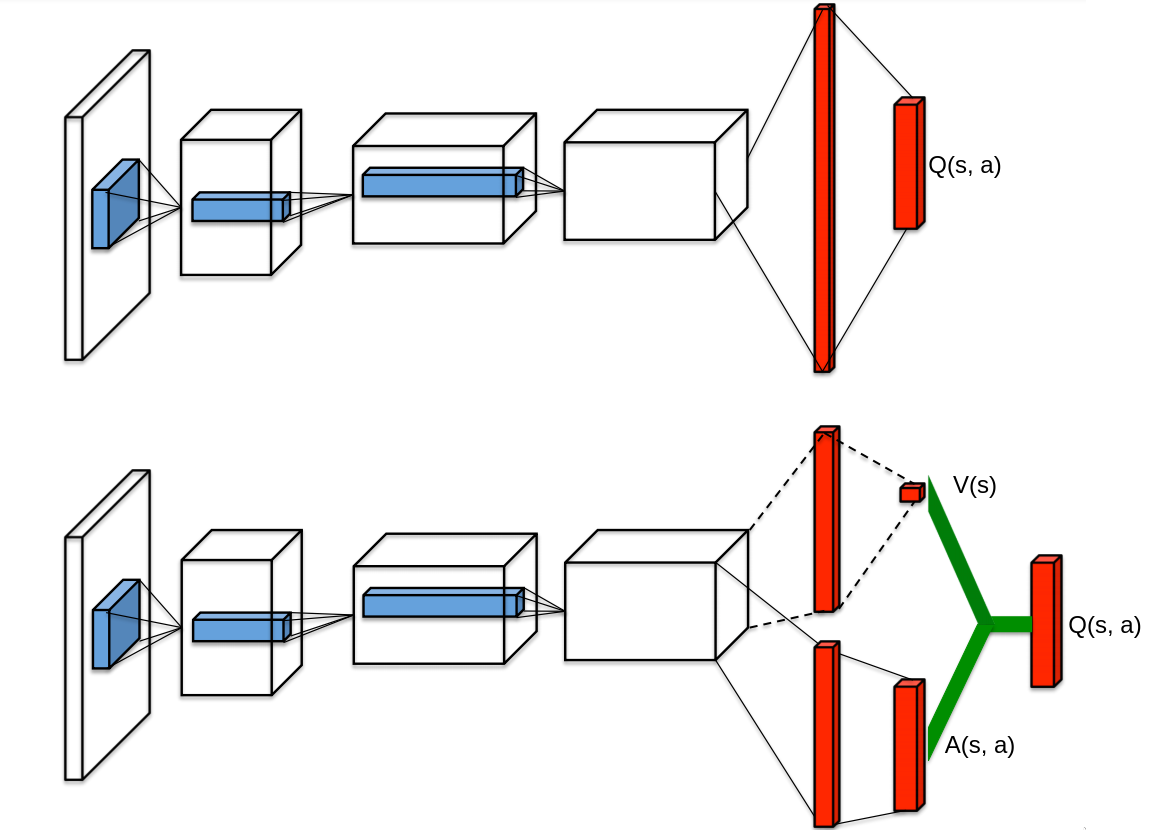
\includegraphics[width=\textwidth]{images/duelingDQN.png}
  \caption{Dueling DQN architecture (bottom) comparison with normal DQN (top), taken from \cite{duelingDQN}.} \label{duelDQNImag}
\end{figure}

\subsection{Asynchronous Advantage Actor-Critic (A3C)}\label{A3C}
\noindent Actor-critic methods try to combine the benefits of both value-iteration methods, like Q-learning and policy-iteration methods, like Policy Gradient, by separating the agent as an actor network and a critic network. The actor network contains the policy that maps states to actions by a set of parameters $\theta$. While the critic network evaluates the value function $V(s)$, the action-value $Q(s,a)$ or the advantage of an action $A(s,a)$, and, based on the \acrshort{TD}-error updates both the actor network and itself. In the case of the \acrshort{A3C}, presented in \cite{a3c}, the critic network tries to estimate the $V(s)$, and the actor network tries to estimate the policy, $\pi(s)$ by maintaining a shared network with two streams like in the case of \acrshort{Dueling DQN}, \cite{duelingDQN}. A diagram showcasing the A3C architecture is shown in Figure \ref{A3CImag}.

The gradient of the loss function can then be defined as:
\begin{equation}
    \nabla L(\theta) = \nabla_{\theta'} log\pi(a_t|s_t; \theta')A(s_t, a_t; \theta, \theta_v) .
\end{equation}

Advantage can be defined as in Equation (\ref{Qfunction}), and by using the relationship between the $Q$ and the $V$ functions from the Bellman optimality equation, the following relationship can be established:

\begin{equation}
    Q(s_t, a_t) = E[r_{t+1} + \gamma V(s_{t+1})] ,
\end{equation}

\begin{equation}
    A(s_t, a_t; \theta, \theta_v) = \sum\limits_{i=0}^{k-1} \gamma^i r_{t+i} + \gamma^k V(s_{t+k}; \theta_v) - V(s_t;\theta_v),
\end{equation}

where $k$ is the number of steps used to the compute new update and $\gamma$ is the discount-rate. This bypasses the need for multiple neural networks as $Q$ and $V$ function approximators.

\begin{figure}[h]
  \centering
  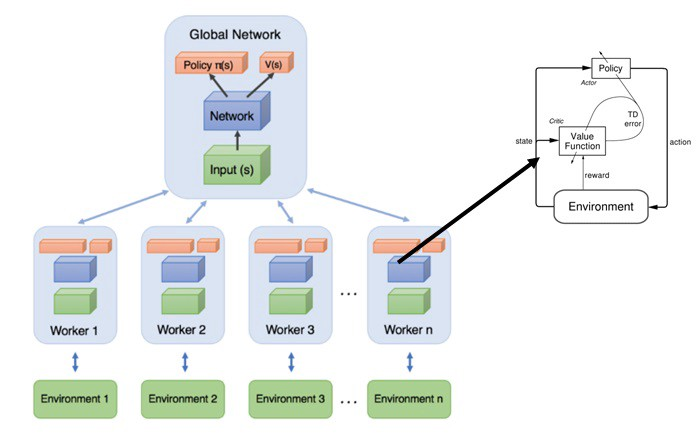
\includegraphics[width=\textwidth]{images/A3C.png}
  \caption{Asynchronous Advantage Actor-Critic (A3C) architecture, taken from \cite{A3CImag}.} \label{A3CImag}
\end{figure}

The main difference between the \acrshort{A3C} method and the alternative \acrshort{A2C} method proposed in \cite{openaia2c} and \cite{a2c} is that in \acrshort{A3C} each worker works independently from other workers running $k$ number of experiences and then computing the gradient and updating with a central network asynchronously, whereas in \acrshort{A2C} there is a synchronization step where each worker waits for all workers to finish their segments of experience and compute their gradient before updating the central network. Also of note, the authors of the \acrshort{A2C} architecture tested if the distributed asynchronous nature of the \acrshort{A3C} network gave it better performance given the stochastic nature of its updates but found no such advantage. The \acrshort{A2C} method runs more effectively when using single \acrshort{GPU} machines, which perform best on large batch sizes of similar computations.


\section{Exploitation vs Exploration} \label{section:EE}
\noindent One major challenge a \acrshort{RL} agent faces is the exploration vs exploitation dilemma. Given a fixed set of resources that must be allocated between competing choices in a way that maximizes expected reward in an unknown transition probability and reward signal environment, the agent must choose to perform actions that exploit known strategies versus performing unknown actions to explore the environment for better strategies. These types of problems have been studied extensively as multi-armed bandit problems.

\subsection{$\epsilon$-greedy algorithm}
\noindent The most common algorithm used to solve this dilemma is the $\epsilon$-greedy algorithm in which the agent performs a greedy selection of the best action most of the times with a $\epsilon$ probability of choosing a random action.

The best action, in the case of a Q-learning algorithm, can be defined as:

\begin{equation}
    a^* =\arg\max\limits_{a} Q(s, a).
\end{equation}

Where in the case of an actor-critic method like A3C, it can be defined as:

\begin{equation}
    a^* =\arg\max\limits_{a} A(s, a).
\end{equation}

To guarantee sufficient exploration at the beginning versus convergence of the \acrshort{RL} agent policy at the end of the training, usually, the $\epsilon$ value shrinks as training goes on. This reflects the intuition that as training goes on, the model becomes better at understanding the environment and the effects of its actions which in turn makes the need to explore less important.

\subsection{Boltzmann exploration} \label{boltz}
\noindent As explained in paper \cite{boltz}, the Boltzmann exploration policy is widely used in \acrshort{RL} problems. The main idea of this algorithm is to build a Boltzmann distribution where instead of using the state's energy, the evaluation of the quality of an action, $Q(s,a)$, in the case of Q-learning algorithms or its advantage, $A(s,a)$, in the case of the \acrshort{A3C} algorithm is used. The probability of choosing each action can be defined according to:

\begin{equation}
    p_i = \frac{e^{-\varepsilon_i/\tau}}{\sum\limits_{j=1}^M e^{-\varepsilon_j/\tau}},
\end{equation}

where $\varepsilon$ is the value of the action, $M$ is the total number of actions and $\tau$ is a hyper-parameter usually called temperature that defines a spectrum between picking the optimal action or a completely random action. When the $\tau$ parameter is close to zero, the Boltzmann policy becomes like the greedy policy, picking the highest valued action. Instead, when the $\tau$ parameter is high, the probability is more widely distributed between other actions. 

As with the $\epsilon$-greedy, this $\tau$ parameter usually shrinks as training goes on, reflecting the intuition that exploration becomes less important as the agent learns the environment.

\subsection{Adaptive Genetic Algorithm (AGA)} \label{AGA}
\noindent In \acrshort{RL} problems with high-dimensional action spaces, methods like the $\epsilon$-greedy policy are very inefficient in their exploration of the environment. To address this problem, the authors of \cite{AGAcrypto} propose an \acrfull{AGA} to make optimal policy convergence faster by reducing useless exploration without reducing performance.

The main idea behind \acrshort{AGA} is to try to use the critic network to evaluate expected reward for each state-action. The presented solution in \cite{AGAcrypto} is a Q actor-critic architecture where the \acrshort{AGA} takes as input the output action from the actor network. A diagram for the proposed architecture can be seen in Figure \ref{AGAcryptoImag}.

If the loss of the critic network is larger than a defined hyper-parameter, $\varphi$, it is assumed that the critic network cannot evaluate actions very well so a random action is generated. This $\varphi$ hyper-parameter can be set as the convergence loss obtained by pre-training the critic network.

\begin{figure}[h]
  \centering
  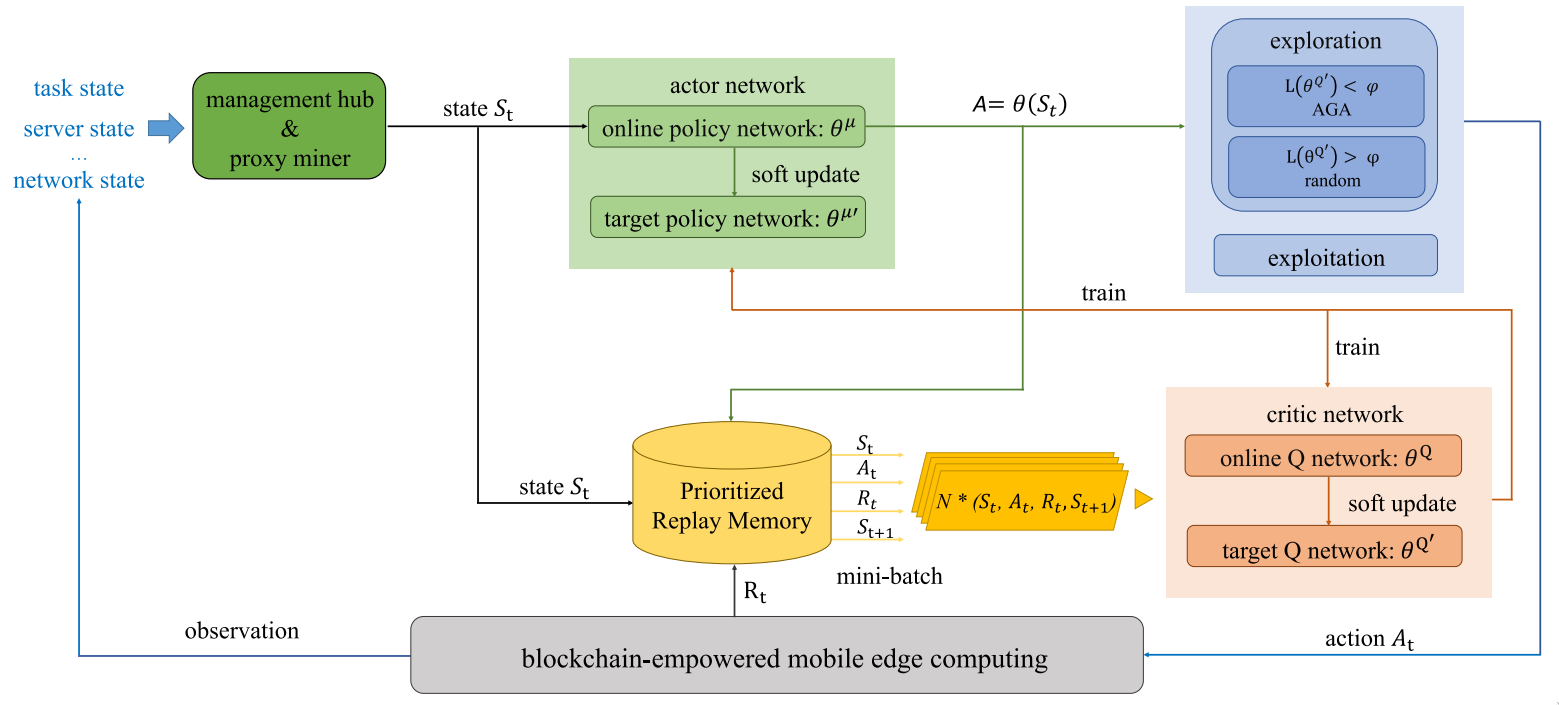
\includegraphics[width=\textwidth]{images/AGA.png}
  \caption{Actor-critic with AGA from \cite{AGAcrypto}.} \label{AGAcryptoImag}
\end{figure}

When the critic network can evaluate the state-action pairs, the \acrshort{AGA} works by taking the output action, $A$, from the actor network and generating $m-1$ random actions obtaining an initial population of candidate solutions of size, $m$, where each action is considered an individual of the population. The genetic operators of crossover and mutation can then be used to create different generations of actions. Using the critic network evaluation as the fitness function in roulette wheel genetic selection, the best actions are selected, and the new generation replaces the population.

The crossover and mutation genetic operators are applied according to their respective probabilities $p_c$ and $p_m$.
\begin{equation}
  p_c =
    \begin{cases}
      \frac{k_1(R_{min}-R')}{\overline{R} - R_{min}} & R' \leq R_{min}\\
      k_3 & R' > R_{min}
    \end{cases},
\end{equation}

\begin{equation}
  p_m =
    \begin{cases}
      \frac{k_2(R-R_{min})}{\overline{R} - R_{min}} & R \geq R_{min}\\
      k_4 & R < R_{min}
    \end{cases},       
\end{equation}

where $\overline{R}$ and $R_{min}$ are the average and minimum values of the population, respectively. These parameters are used to increase $p_c$ and $p_m$ when the population converges to a local minimum. In order to combat disruptions in the global minimum solution, $p_c$ should depend on its parent action value $R'$ and $p_m$ should depend on the value of the mutating action. $k1$, $k2$, $k3$ and $k4 < 1$ are hyper-parameters that define how much crossovers and mutations should happen.

\acrshort{AGA} ends when a $K$ number of iterations are reached and the highest valued action, $A^*$, is selected. This $K$ value can be adapted by:

\begin{equation}
  K =
    \begin{cases}
      \max(0, K-1) & A^* = A\\
      \min(K + \phi(||A-A^*||_2 ), K_{max}) & A^* \neq A
    \end{cases}.
\end{equation}

Where $\phi$ is a strictly monotonically increasing function and $K_{max}$ is an upper limit on the number of generations. 

\section{Related work} \label{section:RW}

\noindent In order to understand the state of the art in solving \acrshort{MEC} challenges using \acrshort{RL}, several works were reviewed. Their problem statements and solutions are summarized in the following sections.

\subsection{User side task offloading}
\noindent Research papers such as \cite{taskclass1} and \cite{taskclass2} present a local offloading decision algorithm that considers a 1 \acrshort{UE} to 1 \acrshort{MEC} server topology in a 4G environment, where the \acrshort{UE} has information about the required computation graph of its application and makes decisions on which computations to offload and which computations to execute locally. 

In \cite{taskclass1}, the algorithm takes a sequentially dependent list of application computation components  and classifies each one as local or remote execution. It assumes that each component's input data amount depends on the output data of the component preceding it and tries to estimate its work as a function of input data and computation complexity as presented in:

\begin{equation} 
    W_c = V \cdot O_n \cdot d_{c-1, c}, 
\end{equation}\label{wcv}

where $W_c$ is the \acrshort{CPU} clock cycles of the computation component ($c_n$), V denotes the number of clock cycles a processor will perform per byte, $O_n$ is the computation complexity of $c_n$ and $d_{c-1,c}$ is the output data amount of the previous component. The $O_n$ notation is introduced as the data amplification factor of $c_n$, given that the input data and the processed data are not equal in amount since the input data can be processed several times.

This paper takes into account the time required to do the computation locally, the transfer delay of uploading input data to the \acrshort{MEC} server defined in Equation (\ref{uploaddelay}) and the transfer delay of the downloading of output data defined in Equation (\ref{downloaddelay}):

\begin{equation}\label{uploaddelay}
r_u = n \frac{B}{N} log_2(1+\frac{p_u|h_{ul}|^2}{\Gamma(g_{ul})d^\beta N_0}),
\end{equation}

\begin{equation}\label{downloaddelay}
r_d = n \frac{B}{N} log_2(1+\frac{p_d|h_{dl}|^2}{\Gamma(g_{dl})d^\beta N_0}),
\end{equation}

where B is the bandwidth, $\beta$ is the path loss exponent, $d$ is the distance between the \acrshort{UE} and the \acrshort{MEC} server, $n$ is the number of subcarriers that are allocated for the transmission, $N_0$ is the noise power, $p_u$ and $p_d$ are the transmit powers, $h_{ul}$ and $h_{dl}$ are the channel fading coefficient for uplink and downlink, and $g_{ul}$ and $g_{dl}$ are the required bit error rate for the uplink and downlink. The SNR margin, $\Gamma$, required to satisfy the bit error rate ($g_{ul}$ and $g_{dl}$) with quadrature amplitude modulation constellation, can be calculated according to:
\begin{equation} \label{SNR}
    \Gamma(g_{l}) = \frac{-2log5g_{ul}}{3} .
\end{equation}

Data is only transferred as it is needed. This means that when two sequential components are offloaded to the \acrshort{MEC} server, the output of the first component is needed as input for the second component. However, since they were both computed on the same machine, there are no upload or download delays between the two.

The proposed classification algorithm is a Deep Neural Network (DNN) trained using the exhaustively computed best solutions from 10,000 randomly generated states for an application consisting of 100 sequential components. This training method quickly becomes intractable for higher complexity problems.

This work does not take into account energy costs of transmission, idle energy costs of waiting for remote computation execution, assumes sequential data dependency in the execution graph and constant \acrshort{CPU} allocation from the \acrshort{MEC} server. 

\subsection{Centralized Fog Network managers}
\noindent Paper \cite{centralfog} presents a centralized \acrfull{SDN} controller which maintains global knowledge of the network of fog nodes. Each fog nodes receives requests from \acrshort{UE}s, and the \acrshort{SDN} controller decides if these tasks should be computed on the receiving node or offloaded to a neighboring node.

This problem statement is formalized as an \acrshort{MDP}, consisting of a state-space (S), action-space (A), transition probability distribution (P) and a reward (R).

\begin{itemize}
    \item $S = \{s=(n^l, w, Q)\}$ is the state space:
    \begin{itemize}
        \item $n^l \in \mathbb{N}$ $(1\leq n^l \leq N)$, is the fog node requested for tasks by end users;
        \item $w \in \mathbb{N} (1 \le w \le W_{max})$, is the number of requested tasks per unit time;
        \item $Q = \{(Q_1,...,Q_N)|Q_i\in\{0, 1,...,Q_{i,max}\}$, is the number of tasks in the node's queue.
    \end{itemize}
    \item $A = \{a=(n^0, w^0)\}$ is the action space:
    \begin{itemize}
        \item $n^0 \in \mathbb{N}$ $(1 \le n^0 \le N, n^0 \ne n^l)$, is a neighboring node to which node $n^l$ is going to offload to;
        \item $w^0 \in \mathbb{N}$ $(1 \le w^0 \le W_{max})$, is the number of tasks to be offloaded to the neighboring node $n^0$. A node can only offload to nodes with an equal or less number of tasks currently requested. The tasks not offloaded are computed locally ($w^l)$.
    \end{itemize}
    \item $P:S \times A \times S \rightarrow [0, 1]$, is the transition probability distribution $P(s'|s,a)$ of a new state $s'$ given that the system is in state $s$ and action $a$ is chosen.
    \item $R:S\times A \rightarrow \mathbb{R}$, is the reward of the system in state $s$ and action $a$ is taken.
    \begin{itemize}
        \item $R(s,a) = U(s, a) - (D(s,a) + O(s,a))$:
        \begin{itemize}
            \item $U(s, a) = r_u log(1+w^l + w^0)$, is the immediate utility and where $r_u$ is a utility reward;
            \item $D(s,a) = \chi_{d} \cdot \frac{t^w + t^c + t^e}{(w^l + w^0)}$ , is the immediate delay and where $t^w$is the average wait time at queue of node $n^l$ and the node $n^0$, $t^c$ is the communication delay between nodes and $t^e$ is the execution time by node $n^l$ and  $n^0$. The $\chi_d$ is a hyper-parameter that defines importance of the delay;
            \item $O(s, a) = \chi_{0} \cdot \frac{w^l \cdot P_{overload, l} + w^0 \cdot P_{overload, 0}}{w^l + w^0}$, is the overload probability and where $\chi_{0}$ is an overload weight hyper-parameter and $P_{overload, i}$ is the task arrival rate at node.
        \end{itemize}
    \end{itemize}
\end{itemize}

To solve this \acrshort{MDP}, the authors of this work propose a Q-table approach using the $\epsilon$-greed algorithm as its policy, which makes its solution not very scalable to higher dimensional problems and makes it suffer from action value overestimation in noisy environments.

This work does not consider the possibility of local \acrshort{UE} task execution and associated battery and computation constraints nor the delay in returning computation results from fog nodes back to the user device.  It also assumes independence between tasks. Despite mentioning the possibility of software-defined fog nodes to be composed of many heterogeneous devices, this is not explored.


\subsection{Decentralized Fog Network managers}
\noindent Paper \cite{fogmulti} continues the work of paper \cite{centralfog} by introducing a new architecture with two important concepts. First, it introduces the notion of dividing the computation resources of fog nodes into network slices, allowing for the allocation of certain slices to services with specific latency and resource requirements. The second important change it makes in its architecture is the change from a centralized \acrshort{SDN} controller with knowledge of the entire network conditions to many distributed controllers located at each fog node working together.

This new problem can be formulated as a \acrshort{POMDP} in which each fog node only knows its local state and makes decisions on which tasks to offload, where to offload them and how to allocate local slices resources to queued tasks. By doing this, no state messages are sent between fog nodes and only locally computed rewards are shared between them. These reward messages can be shared asynchronously from the decision process.

As a solution, each fog node has a \acrfull{DRQN} that takes as input a local observation stack of the previous four observations and makes a local offloading and resource allocation decision. A variation of the $\epsilon$-greedy algorithm is used in which the $\epsilon$ is reset to the starting value with a small decay $\delta^\epsilon$ $(0<\delta^\epsilon < 1)$ every $R^\epsilon$ steps to solve the insufficient exploration in large state-action spaces that $\epsilon$-greedy algorithm suffers from. These neural networks are trained with the experience replay technique trying to maximize the total system reward composed of the local fog node rewards resulting from their localized actions and their effect on the system as a whole.

The work presented in \cite{Lulu}, builds on the work done in \cite{fogmulti} by substituting the fog node's \acrshort{DRQN}s by an \acrshort{A2C} architecture with an actor for each network but a common critic estimator for all agents. This critic needs to be updated with all actions and states from each of the fog nodes but can do so asynchronously from the decision process.

\subsection{Centralized MEC controller}
\noindent Finally, the work presented in \cite{NUE1mec} present a central decision algorithm that makes offloading and resource allocation decisions between a network of \acrshort{UE}s and one \acrshort{MEC} server, as represented in Figure \ref{centralizedMECnetwork}. The algorithm takes as input a list of all tasks that need to be computed by \acrshort{UE}s at that time step and makes a decision of which tasks should be computed on the \acrshort{UE} and which should be offloaded to the \acrshort{MEC} server. It also decides how much of the \acrshort{MEC} server's computation power should be allocated to each offloaded task.

It assumes that each \acrshort{UE} $n$ has a computation-intensive task $R_n \triangleq (B_n, D_n, \tau_n)$ at each time step to be executed, where $B_n$ represents the input data for the computation, $D_n$ represents the total number of \acrshort{CPU} cycles required to compute the task and $\tau_n$ represents the maximum delay amount of that task.

This decision takes into account the delay and energy costs of computing locally, the delay of transmission to the \acrshort{MEC} server, the energy needed to transmit and the idle energy consumption of the \acrshort{UE} when waiting for the remote computation. Due to the assumption of a very high download rate and smaller size of output data than input data, this work ignores the delay and energy cost of downloading the processed result from the \acrshort{MEC} server to the \acrshort{UE}. To solve the problem statement, the authors present a simple \acrshort{DQN}.

\begin{figure}[h]
  \centering
  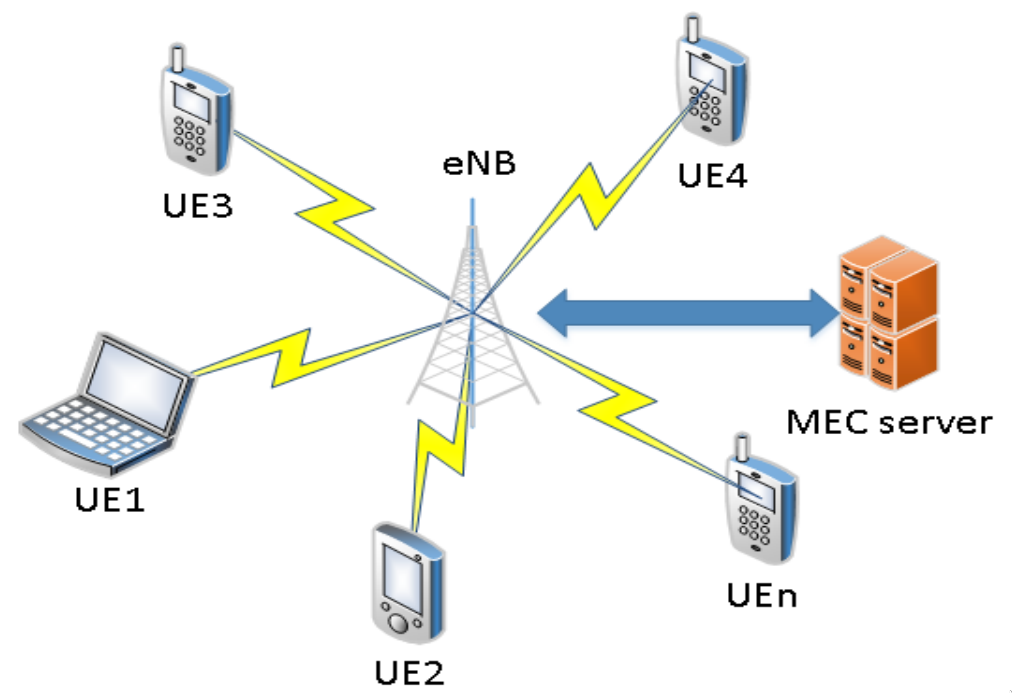
\includegraphics[width=\linewidth]{images/centralizedMECnetwork.png}
  \caption{Network model from \cite{NUE1mec}.} \label{centralizedMECnetwork}
\end{figure}

\chapter{Thesis proposition}

\section{Problem statement}
\noindent The goal of this thesis is the design of a management agent capable of making offloading decisions from an heterogeneous network of \acrshort{UE}s to an heterogeneous network of \acrshort{MEC} servers. This work proposes to innovate by presenting a more complete system and exploring a network topology not present in related works. The proposed network manager could be seen as the conductor in the CONCERT architecture proposed in \cite{CONCERT} or the small cell manager in the \acrshort{SCC} architecture, \cite{SESAM}. This manager would be deployed locally and would manage a group of $M$ \acrshort{MEC} servers and $N$ \acrshort{UE}s making offloading decisions on which \acrshort{UE} tasks to compute locally, which tasks to offload, where tasks should be offloaded to and how the resources of \acrshort{MEC} servers should be allocated. This decision should take into account communication delays, computation constraints and battery consumption.

% TODO: better describe innovation and why it is useful
Building upon the system presented in \cite{NUE1mec}, a system model is defined and the problem is formulated as a \acrshort{MDP}. Finally, \acrshort{DRL} techniques are explored in order to train an optimal network manager.

\subsection{System Model}
\noindent The proposed network model considers N \acrshort{UE}s and M \acrshort{MEC} servers. The set of \acrshort{UE} is denoted as $\mathcal{N} = \{1, 2, ..., N\}$ while the set of \acrshort{MEC} servers can be denoted as $\mathcal{M} = \{1, 2, ..., M\}$. For simplicity \acrshort{MEC} servers are assumed to be connected to the power grid so their energy consumption is ignored.
\begin{itemize}
\item Each \acrshort{UE}, $n \in \mathcal{N}$ can be described by its computation capacity, $f_n^l$ (\acrshort{CPU} cycles per second), transmission power, $P_n$, idle power consumption, $P^i_n$, download power consumption, $P_n^d$, and location, $loc_n = (x_n, y_n, z_n)$. The UE, $n$, can then be described by the vector, $u_n = [f_n^l, P_n, P_n^i, P_n^d, loc_n]$, and the system's \acrshort{UE}s can be defined as the vector $U = [u_1, u_2, ..., u_n]$.

\item Each \acrshort{MEC} server, $m \in \mathcal{M}$, can be described by its computation capacity, $F_m$ (\acrshort{CPU} cycles per second), its transmission power, $P_m$, and its location $loc_m = (x_n, y_n, z_n)$. The \acrshort{MEC} server, $m$, can then be described by the vector, $s_m = [F_m, P_m, loc_m]$ and the system's \acrshort{MEC} servers can be defined as the vector $S = [s_1, s_2, ..., s_n]$.

\item At each time step each \acrshort{UE} is assumed to have a computation task to be completed. This task can either be computed locally or offloaded to one of the available \acrshort{MEC} servers. The offloading decision of each computation task is denoted as $\alpha_n \in \{0, 1, ..., M\}$, where $\alpha_n = 0$ means local computation and $\alpha_n \in \mathcal{M}$ means offloading the task to \acrshort{MEC} server $m = \alpha_n$. The total offloading decision can be defined as the decision vector $\mathcal{A} = [\alpha_1, \alpha_2, ..., \alpha_N]$ with a decision for each task.

\item Each computation task, $R_n$, can be defined by an input data amount, $B_n$ (bits), an output data amount, $B_d$ (bits), the total number of \acrshort{CPU} cycles required to compute it, $D_n$, its maximum allowed delay, $\tau_n$ and the importance weights of time and energy costs, $I_n^t$ and $I_n^e$. The importance weights of the task must satisfy $0 \leq I_n^t \leq 1$, $0 \leq I_n^e \leq 1$ and $I_n^t + I_n^e = 1$. The task, $R_n$, can then be described by the vector, $R_n = [B_n, B_d, D_n, \tau_n, I_n^t, I_n^e]$ and the system's tasks can be defined as the vector $R = [R_1, R_2, ..., R_N]$. 


\end{itemize}

If the network manager decides to compute the task, $R_n$, of \acrshort{UE} $n$ locally then a local computation model can be defined by a local execution delay $T_n^l$ and an energy consumption $E_n^l$:

\begin{equation}
    T_n^l = \frac{D_n}{f_n^l},
\end{equation}

\begin{equation}
    E_n^l = z_n D_n,
\end{equation}

where $z_n$ represents the energy consumption per \acrshort{CPU} cycle and is set to $z_n = 10^{-27}(f_n^l)^2$ according to practical observations made in \cite{energycons}.

Based on the computation delay and energy consumption of task, $R_n$, a local cost can be calculated according to:

\begin{equation}\label{localCost}
    C_n^l = I_n^t T_n^l + I_n^e E_n^l .
\end{equation}

If the network manager decides to offload the computation to the \acrshort{MEC} server $m = \alpha_n$, then the offload computation model can be defined by an upload delay, $T_{n,t}^m$, an upload energy consumption, $E_{n,t}^m$, an offload execution delay, $T_{n,p}^m$, an idle energy consumption, $E_{n,p}^m$, a download delay, $T_{n,d}^m$ and its corresponding download energy consumption, $E_{n,d}^m$.

Firstly, the \acrshort{UE} $n$ must upload the input data, $B_n$ from the task $R_n$ to the decided \acrshort{MEC} server $m$. This upload has an associated delay defined as:

\begin{equation} \label{transmission_delay}
    T_{n,t}^m = \frac{B_n}{r_u},
\end{equation}

where $r_u$ is the uplink rate of \acrshort{UE} $n$ computed according to Equation (\ref{uploaddelay}) from \cite{taskclass1} and the distance, $d_n^m$, between the \acrshort{MEC} server $m$ and the \acrshort{UE} $n$ can be calculated using the euclidean norm between their locations.

\begin{equation} \label{distance_nm}
    d_n^m = ||loc_m - loc_n||_2
\end{equation}

This upload has an associated energy consumption:

\begin{equation} \label{transmission_energy}
    E_{n,t}^m = P_n T_{n,t}^m = \frac{P_n B_n}{r_u} .
\end{equation}

After the data is uploaded the \acrshort{MEC} server then computes the task resulting in a offload execution delay:

\begin{equation} \label{processing_delay}
    T_{n,p}^m = \frac{D_n}{f_m} ,
\end{equation}

where $f_m$ is the amount of the \acrshort{MEC} server, $m$, computation capacity, $F_m$, allocated to the offloaded task. To simplify the system the computation capacity of a \acrshort{MEC} server is equally divided by all tasks offloaded to it:

\begin{equation}
    f_m = \frac{F_m}{N_m}, 
\end{equation}

where $N_m$ is the number of tasks offloaded to \acrshort{MEC} server, $m$.

While the \acrshort{UE} waits for the task to be computed it stays idle which has an associated energy consumption:

\begin{equation} \label{idle_energy}
    E_{n,p}^m = P_n^i T_{n,p}^m = \frac{P_n^i D_n}{f_m}.
\end{equation}

Finally the computation results are downloaded to the \acrshort{UE} $n$ with an associated delay:

\begin{equation} \label{download_delay}
    T_{n, d}^m = \frac{B_d}{r_d},
\end{equation}

where $B_d$ is the size of the computation output and $r_d$ is the download rate of \acrshort{UE} $n$ according to the Equation (\ref{downloaddelay}) from \cite{taskclass1}. 

This download step has an associated energy consumption that can be calculated according to:

\begin{equation} \label{download_energy}
    E_{n, d}^m = P_n^d T_{n, d}^m .
\end{equation}

By taking into account the delays defined in Equations (\ref{transmission_delay}), (\ref{processing_delay}) and (\ref{download_delay}), we can compute the total offload delay, $T_n^m$ as the sum of all delays:

\begin{equation}
    T_n^m = T_{n,t}^m + T_{n,p}^m + T_{n, d}^m .
\end{equation}

The total energy consumption of offloading to the \acrshort{MEC} server $m$, can be calculated by adding all energy consumptions defined in Equations (\ref{transmission_energy}), (\ref{idle_energy}) and (\ref{download_energy}):

\begin{equation}
    E_n^m = E_{n,t}^m + E_{n,p}^m + E_{n, d}^m .
\end{equation}

Based on the computation delay and energy consumption of offloading task $R_n$ to \acrshort{MEC} server $m$, a cost can be calculated according to:

\begin{equation}
    C_n^m = I_n^t T_n^m + I_n^e E_n^m .
\end{equation}

The cost of the offloading decision $\alpha_n \in \{0, 1, ..., M\}$ can be computed according to:

\begin{equation}
    C_n =     
    \begin{cases}
      C_n^l & \alpha_n = 0\\
      C_n^m & \alpha_n \in \mathcal{M}
    \end{cases} .
\end{equation}

The sum cost of the \acrshort{MEC} system at each iteration can then be defined as:

\begin{equation}
    C_{all} = \sum\limits_{n=1}^N C_n .
\end{equation}

For checking the delay constraint, $\tau_n$, the total delay, $T_n$, of the offloading decision $\alpha_n$ can is defined as:

\begin{equation}
    T_n =     
    \begin{cases}
      T_n^l & \alpha_n = 0\\
      T_n^m & \alpha_n \in \mathcal{M}
    \end{cases} .
\end{equation}

\subsection{Problem formulation}
% TODO: Update problem formulation with worst case formulation
\noindent The offloading decision can then be formulated as the following optimization problem:

\begin{mini*}|s|
{\mathcal{A}}{\sum\limits_{n=1}^N C_n}
{}{}
\addConstraint{C1: \alpha_n \in \{0, 1, ..., M\}, \forall n \in \mathcal{N}}
\addConstraint{C2: T_n \leq \tau_n, \forall n \in \mathcal{N}}
\end{mini*}

This optimization function has the objective of finding the offloading decision vector $\mathcal{A} = [\alpha_1, \alpha_2, ..., \alpha_n]$ that minimizes the sum cost of the system at each time step.

\subsection{Solution}
\noindent Given the complex nature of the proposed problem and the lack of perfect knowledge of network conditions this thesis proposes to use a model-free \acrshort{DRL} agent to manage the network. This means that the network manager does not have access to the transition probability, $P(s_{t+1}|s_t, a_t)$, nor the reward function $R(s, a)$ and must learn them by experimenting on the environment.

To do this the problem is formulated as an \acrshort{MDP}, $<S, A, P, R>$:
\begin{itemize}
    \item $S=\{s=(U, S, R)\}$ is the state space, which contains all \acrshort{UE} states, $U$, \acrshort{MEC} server states, $S$, and requested tasks, $R$;
    \item $A=\{a=(\mathcal{A})\}$ is the action space, which contains the offloading decision vector for all tasks, $\mathcal{A}$;
    \item $P:S \times A \times S \rightarrow [0, 1]$ is the transition probability distribution $P(s_{t+1}|s_t, a_t)$;
    \item $R = \frac{C_{local} - C(s,a)}{C_{local}}$ is the reward function, which is defined as in \cite{NUE1mec} where it is inversely related to the system cost, $C(s,a)$, normalized by the system cost with only local computation $C_{local}$. 
\end{itemize}

At each time step, $t$, this network manager takes a state, $s_t$, makes a decision, $a_t$, that results in the state, $s_{t+1}$, and a reward $r_t$. The goal is then finding the policy, $\pi$, that maximizes the expected return, $V_\pi(s)$ as defined in Equation (\ref{Vfunction}). 

To achieve this, several \acrshort{DRL} algorithms will be explored: \acrshort{DQN}, \acrshort{DDQN}, \acrshort{Dueling DQN} and \acrshort{A2C}.

\section{Methods and tools}

\noindent In order to implement a network manager capable of dealing with the proposed system two main challenges need to be addressed: 1) the implementation of the \acrshort{DRL} algorithms; 2) the implementation of the proposed system simulator. The programming language that will be used to implement all algorithms and the simulator is Python. The reason behind this decision is that given its popularity as the second most used programming language overall \cite{pythonpop} and the most used in the machine learning context \cite{pythonmachine}, most of all popular \acrshort{DRL} tools are written in Python.

As for the implementation of the \acrshort{DRL} algorithms two main tools were considered, Tensorflow 2.0 \cite{tensorflow} with the Keras API layer and Pytorch \cite{pytorch}. Due to the higher popularity of Tensorflow in the reinforcement learning context it was chosen as the neural network library used to write all DRL algorithms.

The second major challenge is the implementation of the simulator. OpenAI Gym was introduced in \cite{opengym} in order to standardize reinforcement learning environments and benchmarks. Due to its easy integration with Keras demonstrated in \cite{kerasrl} and \cite{kerasrl2} it was chosen as the tool for implementing the simulation environment of the proposed system.

\chapter{Results}
% TODO: Rewrite chapter 4 as results
% 1 - Scalability, fix number of MEC and increase number of UEs
% Show learning, show performance
% 2 - Robustness, change system hyper parameters
% Show leaning and performance
% 3 - Show impact of worst case scenario reward
% Show learning and performance as increasing max weight

\section{Baselines} \label{baselines}
\noindent In order to benchmark the various \acrshort{DRL} algorithms and test the implemented simulator, several baseline algorithms were developed:

\begin{itemize}
    \item Full Local: all \acrshort{UE}s execute their tasks locally, in terms of the decision vector $\mathcal{A}=[0_1, 0_2, ..., 0_N]$. This represents the case where the system has no offloading capabilities.
    \item Random Offload: where the offloading decision is completely random, each task is either executed locally or offloaded to one of the available \acrshort{MEC} servers randomly;
    \item Full nearest \acrshort{MEC}: all \acrshort{UE} tasks are offloaded to the nearest \acrshort{MEC} server according to Equation (\ref{distance_nm}). This represents the case of offloading to the nearest node without regarding their computation constraints and other offloading decisions. This baseline also requires knowledge of the network topology which the agent does not have.
\end{itemize}

The plan is to create several system configurations of increasing complexity. The baseline algorithms will be used in order to benchmark the quality of trained agents. It is expected that the proposed network manager will surpass their performance in all situations by making intelligent decisions taking into account computation, battery, delay and communication constraints, which are ignored by the baselines.

\section{Simple test} \label{simple_test}

To put these baselines, the agent and the simulator to the test, a simple test case was devised. In this test, there are five \acrshort{UE}s and five \acrshort{MEC} servers. The UEs and MEC servers were randomly distributed in a 2D plane with $x \in [0, 200]$ and $y \in [0, 200]$, resulting in the distribution seen in Figure \ref{example_layout}.

\begin{figure}[H]
  \centering
  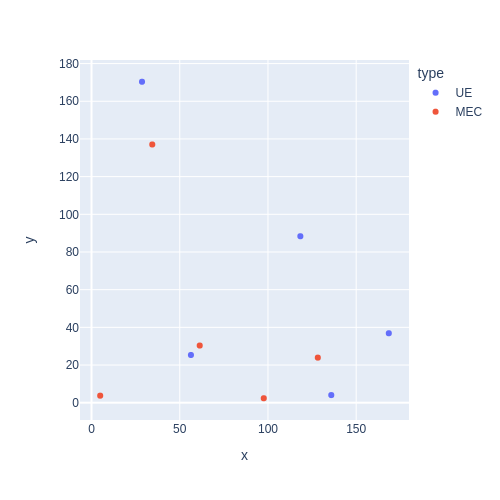
\includegraphics[width=200px]{images/example_layout.png}
  \caption{Example layout for the simple test.}  \label{example_layout}
\end{figure}

For simplicity, all \acrshort{UE}s and \acrshort{MEC} servers are considered to have the same specifications. The system's hyper-parameters were set according to the values present in Table \ref{hyperparams}. In order to test this configuration, the task parameters, $B_n$, $B_d$ and $D_n$ were sampled from uniform distributions between ($300$, $500$) Kbits, ($10$, $15$) Kbits and ($900$, $1100$) Megacyles respectivly. 

% Please add the following required packages to your document preamble:
% \usepackage[normalem]{ulem}
% \useunder{\uline}{\ul}{}
\begin{table}[H]
\centering
\begin{tabular}{|l|l|l|l|}
\hline
Variable             & Value & Variable                & Value \\ \hline
$B$&$10\times10^{6}$&$f_n^l$&$1\times10^{9}$\\
$n$&$10$&$I_n^t$&$0.5$\\
$\beta$&$-4$&$I_n^e$&$0.5$\\
$h_ul$&$100$& $P_m$&$200$\\
$h_dl$&$100$& $P_n$& $500\times10^{-3}$\\
$g_ul$&$1$&$P_n^i$&$100\times10^{-3}$\\
$g_dl$&$1$&$P_n^d$&$200\times10^{-3}$\\
$N_0$&$5\times10^{-5}$&$F_m$&$5\times10^{9}$\\
$W_{mean}$&$1$&$W_{max}$&$0$\\ \hline
\end{tabular}
\caption{System hyper-parameters.}\label{hyperparams}
\end{table}

The agent described in Section \ref{solution} was trained with the following hyper-parameters:

\begin{table}[H]
\centering
\begin{tabular}{|l|l|}
\hline
Variable & Value \\ \hline
episode length&$10$\\
learning rate, $\alpha$&$0.0001$\\
discount factor, $\gamma$&$0.99$\\
batch size&$200$\\ \hline
\end{tabular}
\caption{Training hyper-parameters.}\label{training_hyperparams}
\end{table}

Each algorithm ran for 100 episodes and an average per episode of offloading decisions is shown in Table \ref{resultstest1}.

\begin{table}[H]
\centering
\begin{tabular}{|l|l|l|}
\hline
Algorithm        & Average Reward ($R$) & Reduction\\ \hline
Full Local       & -49.47 & 96.65\%\\
Random Offload   & -9.68 & 82.89\%\\
Full nearest MEC & -2.18 & 24.06\%\\ 
Agent (A2C) & -1.66 & -\\ \hline
\end{tabular}
\caption{Average Reward ($R$) over 100 iterations.} \label{resultstest1}
\end{table}

As expected, the Full Local baseline performed the worst given that it does not make use of the \acrshort{MEC} servers computing capabilities, leading to an increased cost due to increased energy consumption and delay of the tasks. The Random Offload baseline is the second worst, given that although it gains from offloding to \acrshort{MEC} servers, it does so without any consideration for the system's configuration. From the baselines, Full nearest MEC performed the best since it takes into consideration the distance between the \acrshort{UE} and the \acrshort{MEC} server but it comes with the disadvantage of not only requiring knowledge of the network topology (positions of \acrshort{UE}s and \acrshort{MEC}s) but also not taking into account anything else. 

As expected, the proposed agent outperformed the baselines in all situations, which demonstrates that the agent is able to learn not only the topology of the network by trying out different offloading decisions but also make intelligent decisions based on computation, battery, delay and communication constraints ignored by the baselines.

\begin{figure}[H]
  \centering
  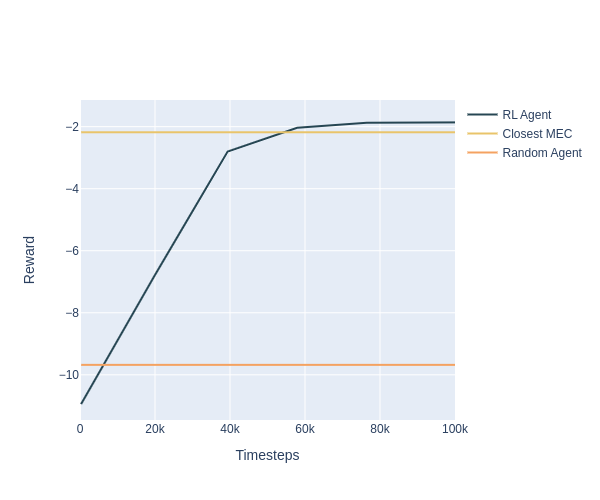
\includegraphics[width=250px]{images/5_5_training.png}
  \caption{Agent reward while training.}  \label{5_5_training}
\end{figure}

As shown in Figure \ref{5_5_training}, the agent starts with an equivelent reward to the Random Offload, which is expected since the agent has not yet learned the environment. As the agent interacts with the environment making offloading decisions (actions), it recieves state transitions and rewards. This allows it to quickly learn the system and the reward increases rapidly in the first iterations. After about 55K steps in the environment, the agent surpasses the best offloading baseline, Full nearest MEC. As expected, the reward starts to stabilize as the agent learns the final details of the system increasing slightly the final performance.

\section{Scalability and Data Efficiency} \label{scalability_data}

In this section the scalability and data efficiency of our agent is explored. Scalability in this context can be defined as the ability of the agent to learn and outperform the baselines in higher complexity problems. 

Data efficiency in this context can be defined as the ability of the agent to learn in as few possible steps as possible. While it is expected that the agent takes longer to learn in more complex problems, the complexity of the underlying policy should not grow linearly with the state and action spaces. The reason for this is that it is expected that the agent is able to generalize concepts instead of brute forcing a solution for each problem set.

Since our state space is defined as the requested tasks at each step and each task is defined by a set of 5 parameters, the complexity of the state space grows linearly with the amount of \acrshort{UE}s, \emph{N}. The size of the state space should be $N \times 5$. 

On the other side, the action space is defined as the offloading decision of each task. Given that each task can be computed locally or offloaded to one of the \acrshort{MEC} servers, \emph{M}, this gives us the option of $M + 1$ actions per task. This results in the action space growing exponentially with the amount of \acrshort{UE}s, \emph{N}, since there are $(M + 1)^N$ possible actions at each decision step.

With this in mind, the stability and data efficieny of the system can be tested by setting the system's hyper-parameters and amount of \acrshort{MEC} servers to be the same as in the simple test case and create two new test scenarios by increasing the number of \acrshort{UE}s to 10 and 20, respectively.

The UEs and MEC servers were randomly distributed in a 2D plane with $x \in [0, 200]$ and $y \in [0, 200]$, resulting in the distribution seen in Figure \ref{5_10_layout} and Figure \ref{5_20_layout}.

\begin{minipage}{0.5\textwidth}
\begin{figure}[H]
  \centering
  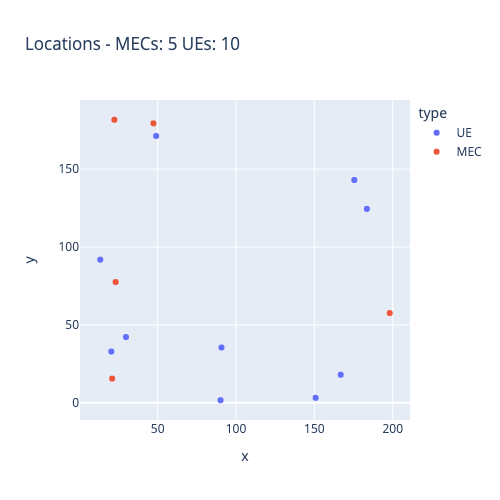
\includegraphics[width=200px]{images/5_10_layout.png}
  \caption{Test with 10 \acrshort{UE}s.}  \label{5_10_layout}
\end{figure}
\end{minipage}
\begin{minipage}{0.5\textwidth}
\begin{figure}[H]
  \centering
  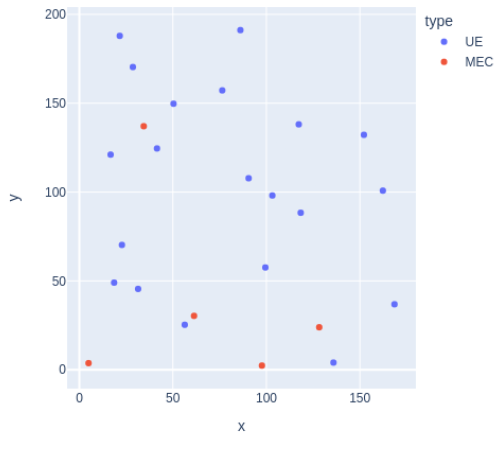
\includegraphics[width=200px]{images/5_20_layout.png}
  \caption{Test with 20 \acrshort{UE}s.}  \label{5_20_layout}
\end{figure}
\end{minipage}

\hfill \break
Each algorithm ran for 100 episodes and an average per episode of offloading decisions is shown in Table \ref{results_5_10} and Table \ref{results_5_20}.

\begin{table}[H]
\centering
\begin{tabular}{|l|l|l|}
\hline
Algorithm        & Average Reward ($R$) & Reduction\\ \hline
Full Local       & -49.50 & 94.40\%\\
Random Offload   & -10.32 & 73.14\%\\
Full nearest MEC & -3.56 & 22.17\%\\ 
Agent (A2C) & -2.77 & -\\ \hline
\end{tabular}
\caption{Average Reward ($R$) over 100 episodes with 10 \acrshort{UE}s} \label{results_5_10}
\end{table}

\begin{table}[H]
\centering
\begin{tabular}{|l|l|l|}
\hline
Algorithm        & Average Reward ($R$) & Reduction\\ \hline
Full Local       & -49.49 & 90.42\%\\
Random Offload   & -11.67 & 59.36\%\\
Full nearest MEC & -7.23 & 34.38\%\\ 
Agent (A2C) & -4.74 & -\\ \hline
\end{tabular}
\caption{Average Reward ($R$) over 100 episodes with 20 \acrshort{UE}s} \label{results_5_20}
\end{table}

As expected, the reward of the Full Local baseline stays almost the same between test environments. This happens because these tests set $W_{mean}$ to 1 and $W_{max}$ to 0, so the cost is only composed by $C_{mean}$, defined in Equation \ref{C_mean}. Since $C_{mean}$ is the average cost of each \acrshort{UE}'s task, this should not scale with the amount of \acrshort{UE}s.

The same cannot be said of the other baselines and the agent. Since the number of \acrshort{MEC}s stays the same and the number of tasks increases, the overall cost of the system increases with the amount of \acrshort{UE}s. This represents the computation constraint of the \acrshort{MEC} servers. 

These results demonstrate that the agent scales with the complexity of the system.

In order to study the data efficiency of the agent, the agent's performance while training must be analysed.


\begin{minipage}{0.5\textwidth}
\begin{figure}[H]
  \centering
  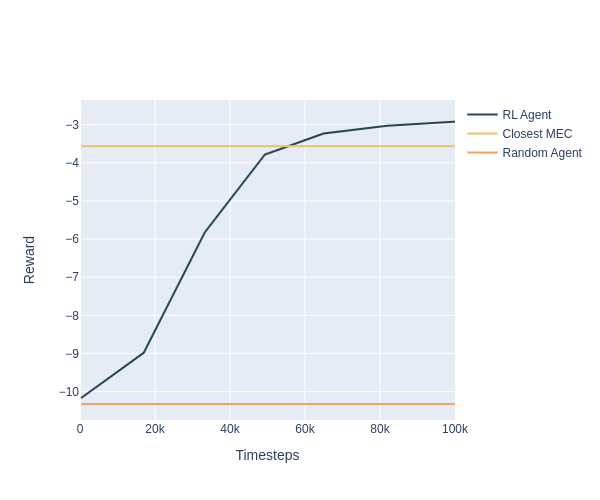
\includegraphics[width=230px]{images/5_10_training.png}
  \caption{Training with 10 \acrshort{UE}s.}  \label{5_10_training}
\end{figure}
\end{minipage}
\begin{minipage}{0.5\textwidth}
\begin{figure}[H]
  \centering
  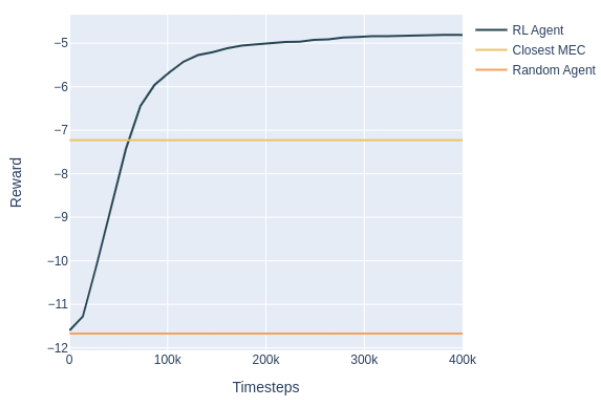
\includegraphics[width=230px]{images/5_20_training.png}
  \caption{Training with 20 \acrshort{UE}s.}  \label{5_20_training}
\end{figure}
\end{minipage}

\hfill \break
The same trend as the simple test can be observed with the two new tests in Figure \ref{5_10_training} and Figure \ref{5_20_training}. The agents starts with an equivelent reward to the Random Offload, then it quickly learns the system and the reward increases rapidly in the first iterations. After about 55K steps in both environments, the agent surpasses the best offloading baseline, Full nearest MEC. As expected, the reward starts to stabilize as the agent learns the final details of the system increasing slightly the final performance.

This confirms that the agent is data efficient, meaning that even when the system's state space increases linearly and the action space increases exponentially, the agent is able to generalize concepts achieving a good performance. It does this with almost the same number of interactions with the system proving it is finding a strategy without brute forcing a solution.

\section{Robustness and Stability} \label{robustness_stability}

In this section the robustness and stability of our agent is explored. Robustness in this context can be defined as the ability of the agent to learn and outperform the baselines in environments with different network conditions and heterogeneous computation capabilities. 

Stability in this context can be defined has the ability of the agent to not diverge or collapse while training. This means that its performance should improve as it interacts with the environment and after learning a strategy it should not forget it, collapsing the system's performance.

In order to test the system's robustness to changing network conditions, a new test case is devised by setting the system hyper-parameters to the values present in Table \ref{new_hyperparams}.

\begin{table}[H]
\centering
\begin{tabular}{|l|l|l|l|}
\hline
Variable             & Value & Variable                & Value \\ \hline
$B$&$10\times10^{6}$&$f_n^l$&$0.75\times10^{9}$\\
$n$&$10$&$I_n^t$&$0.25$\\
$\beta$&$-4$&$I_n^e$&$0.75$\\
$h_ul$&$50$& $P_m$&$100$\\
$h_dl$&$50$& $P_n$& $250\times10^{-3}$\\
$g_ul$&$0.5$&$P_n^i$&$50\times10^{-3}$\\
$g_dl$&$0.5$&$P_n^d$&$100\times10^{-3}$\\
$N_0$&$3\times10^{-5}$&$F_m$&$2.5\times10^{9}$\\
$W_{mean}$&$1$&$W_{max}$&$0$\\ \hline
\end{tabular}
\caption{New system hyper-parameters.}\label{new_hyperparams}
\end{table}

By setting the number of \acrshort{UE}s to 10 and the number of \acrshort{MEC}s to 5, they were randomly distributed in a 2D plane with $x \in [0, 200]$ and $y \in [0, 200]$, resulting in the distribution seen in Figure \ref{robust_test}.

\begin{figure}[H]
  \centering
  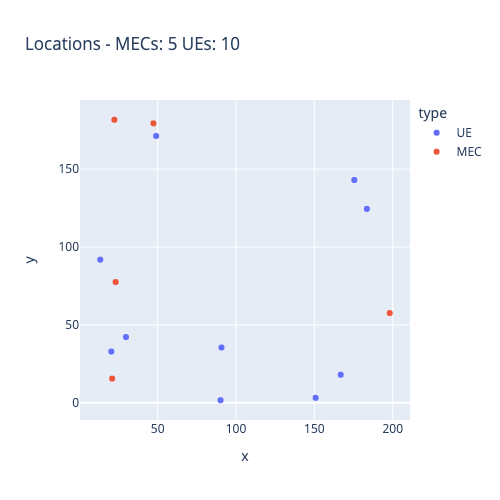
\includegraphics[width=200px]{images/5_10_layout.png}
  \caption{Robustness test layout.}  \label{robust_test}
\end{figure}

Each algorithm ran for 100 episodes and an average per episode of offloading decisions is shown in Table \ref{robust_table}.

\begin{table}[H]
\centering
\begin{tabular}{|l|l|l|}
\hline
Algorithm        & Average Reward ($R$) & Reduction\\ \hline
Full Local       & -31.31 & 84.92\%\\
Random Offload   & -9.14 & 48.35\%\\
Full nearest MEC & -6.81 & 30.62\%\\ 
Agent (A2C) & -4.72 & -\\ \hline
\end{tabular}
\caption{Average Reward ($R$) over 100 episodes of robustness test.} \label{robust_table}
\end{table}

As expected the reward values of all the algorithms differ from previous tests since the system hyper-parameters that are used to calculate the reward function are different.

The same cost reduction trends can be observed in this new environment, showing that the agent is able to learn the system's behaviour independently of the network conditions.

\begin{figure}[H]
  \centering
  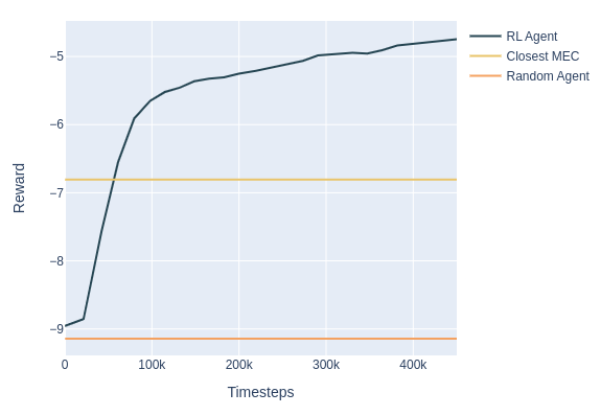
\includegraphics[width=250px]{images/5_10_training_new.png}
  \caption{Training in robustness test.}  \label{robust_training}
\end{figure}

As shown in Figure \ref{robust_training}, the agent's performance while training follows a similar trend to previous tests. The agent starts with an equivelent reward to the Random Offload, then it quickly learns the system and the reward increases rapidly in the first iterations. After about 55K steps, the agent surpasses the best offloading baseline, Full nearest MEC. As expected, the reward starts to stabilize as the agent learns the final details of the system, slightly increasing the final performance.

The other component of robustness that must be tested is robustness to heterogeneous computation capabilities of \acrshort{UE}s and \acrshort{MEC} servers. To test this, a new test case is devised by resetting the system hyper-parameters to the values present in Table \ref{hyperparams} but instead of setting $f^l_n$ and $F_m$ to a fixed value, they are set to a value randomly sampled from a set of values, $f = \{0.25, 0.5, 0.75, 1\} \times 10^9$ and $F = \{2.5, 5, 7, 10\} \times 10^9$, respectively.

By setting the number of \acrshort{UE}s to 10 and the number of \acrshort{MEC}s to 5, they were randomly distributed in a 2D plane with $x \in [0, 200]$ and $y \in [0, 200]$, resulting in the distribution seen in Figure \ref{hetero_test}.

\begin{figure}[H]
  \centering
  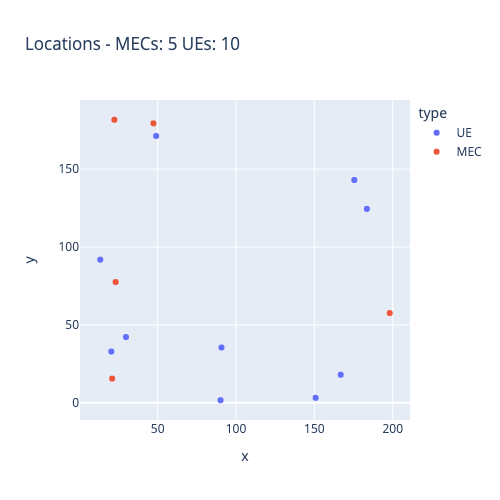
\includegraphics[width=200px]{images/5_10_layout.png}
  \caption{Heterogeneous test layout.}  \label{hetero_test}
\end{figure}

Each algorithm ran for 100 episodes and an average per episode of offloading decisions is shown in Table \ref{hetero_table}.

\begin{table}[H]
\centering
\begin{tabular}{|l|l|l|}
\hline
Algorithm        & Average Reward ($R$) & Reduction\\ \hline
Full Local       & -33.56 & 89.55\%\\
Random Offload   & -8.80 & 60.16\%\\
Full nearest MEC & -5.04 & 30.39\%\\ 
Agent (A2C) & -3.51 & -\\ \hline
\end{tabular}
\caption{Average Reward ($R$) over 100 episodes of heterogeneous test.} \label{hetero_table}
\end{table}

As presumed, the reward values of all the algorithms differ from previous tests since the system computation capabilities that are used to calculate the reward function are different.

Although the ordering of the algorithm performances stays the same in this test case, the cost reduction of our agent in comparison to the Full nearest MEC is higher. With a reported 30.39\% improvement, while the equivelant homogeneous test had an improvement of 22.17\%. This makes sense given that the Full nearest MEC only takes into account the distance of \acrshort{UE}s to \acrshort{MEC}s and not their computation capabilities. This in turn leads to worse load balancing when the computation capabilities of the \acrshort{UE}s and \acrshort{MEC}s are not all the same.

The agent on the other hand is able to learn the system's network topology and make offloading decisions that better load balance the required tasks. 

By analysing all training curves, it is clear that the agent is stable and its reward does not diverge or collapse while trainnig, even when ran for millions of iterations.

\begin{figure}[H]
  \centering
  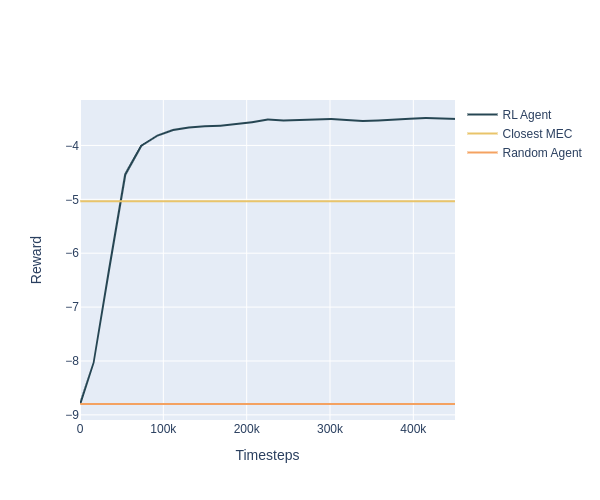
\includegraphics[width=250px]{images/5_10_training_hetero.png}
  \caption{Training in heterogeneous environment.}  \label{hetero_training}
\end{figure}

As shown in Figure \ref{hetero_training}, the agent's performance while training follows a similar trend to previous tests. The agent starts with an equivelent reward to the Random Offload, then it quickly learns the system and the reward increases rapidly in the first iterations. After about 50K steps, the agent surpasses the best offloading baseline, Full nearest MEC. As expected, the reward starts to stabilize as the agent learns the final details of the system increasing slightly the final performance.

\section{Reward function weights} \label{reward_section}

This section focuses on studying the effect of the cost function importance weights on the agent's overall and worst case performance.

To test this, five new test cases were created by setting the system hyper-parameters to the values present in Table \ref{hyperparams} but instead of setting $W_{mean}$ to 1 and $W_{max}$ to 0, they are set to $(1, 0.75, 0.5, 0.25, 0)$ and $(0, 0.25, 0.5, 0.75, 1)$, respectively.

By setting the number of \acrshort{UE}s to 10 and the number of \acrshort{MEC}s to 5, they were randomly distributed in a 2D plane with $x \in [0, 200]$ and $y \in [0, 200]$, resulting in the distribution seen in Figure \ref{weight_test}.

\begin{figure}[H]
  \centering
  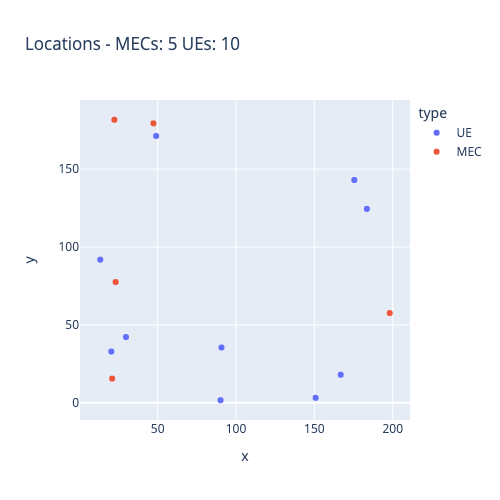
\includegraphics[width=200px]{images/5_10_layout.png}
  \caption{Weight test layout.}  \label{weight_test}
\end{figure}

Each combination of the cost function ran for 100 episodes and an average per episode of offloading decisions is shown in Table \ref{weight_table}.

\begin{table}[H]
\centering
\begin{tabular}{|l|l|l|l|}
\hline
$\{W_{mean}, W_{max}\}$ & Overall Cost & Worst Cost & Difference \\ \hline
$\{1, 0\}$       & 2.72 & 4.04 & 1.32\\
$\{0.75, 0.25\}$  & 2.97 & 3.84  & 0.87\\
$\{0.5, 0.5\}$ & 3.22 & 3.53 & 0.31\\ 
$\{0.25, 0.75\}$ & 3.52 & 3.81 & 0.29\\ 
$\{0, 1\}$ & 3.81 & 3.78 & -0.03 \\ \hline
\end{tabular}
\caption{Agent performance over 100 episodes of weight tests.} \label{weight_table}
\end{table}

As the weights shift from prioritizing overall performance to prioritizing worst case performance, the agent's overall cost increases while the worst case cost decreases. While the agent outperforms the best baseline with every weight distribution, it learns to make offloading decisions that prioritize the worst case performance at the expense of overall system performance. With this in mind, the process of picking the best weight distribution would involve trying to determine the maximum cost allowed per \acrshort{UE} and shifthing the weight distribution in favour of $W_{max}$, trying to maximize $W_{mean}$ while still meeting the maximum allowed cost.


\chapter{Conclusions}
\section{Summary}
% TODO: Update conclusions
\noindent As presented in Chapter \ref{chap:stateoftheart} Section \ref{section:MECarch} several architectures have been proposed in the \acrshort{MEC} context that present complex optimization problems of managing how to distribute tasks between \acrshort{UE}s and \acrshort{MEC} servers. Due to the high dimensional complexity and uncertain networking conditions, classical offline optimization algorithms fail to effectively manage these types of problems. As a solution to this, a review of the state of the art in \acrshort{DRL} and its application to these \acrshort{MEC} challenges was made in Chapter \ref{chap:stateoftheart} Sections \ref{section:RL}, \ref{section:EE} and \ref{section:RW}. Based on the work done by papers \cite{NUE1mec} and \cite{taskclass1} a more complete system that takes into account the possibility of offloading between a network of heterogeneous \acrshort{UE}s to a network of heterogeneous \acrshort{MEC} servers is proposed. As far as the candidate knows, this is the first time that this extended optimization problem is addressed. To deal with the increased complexity of taking into account computation, battery, delay and communication constraints in an N to N problem a network manager agent is proposed in Section \ref{solution}. In order to evaluate the performance of the proposed agent, several baselines are described in Section \ref{baselines}. Finally, the agent's capabilities are put to the test in Sections \ref{simple_test}, \ref{scalability_data}, \ref{robustness_stability} and \ref{reward_section}.

In Section \ref{simple_test}, a simple test case is used to demonstrate the simulator, baselines and the agent's capacity to learn. As expected, the Full Local baseline performs the worst, then the Random Offload baseline and finally the Full nearest MEC. The proposed agent is shown to learn, overperforming the baselines by 96.65\%, 82.89\% and 24.06\% respectively. The agent achieves this while not requiring any information of the network topology by simply interacting with the environment.

In Section \ref{scalability_data}, the agent's scalability and data efficiency is put to the test by increasing the complexity of the system with two new tests. Given that the system complexity is tightly related with the number of \acrshort{UE}s in the network, the agent was tested in an environment with 10 and 20 \acrshort{UE}s. As showcased, the agent learned to overperform the best baseline with a 22.17\% and 34.38\% improvement respectively, showcasing its ability to scale with problem complexity. The agent also achieved this in 55K, demonstrating it's data efficiency.

Section \ref{robust_test} serves to test the agent's robustness and stability. In order to test robustness, two new test cases were implemented. First, the agent robustness to changing network conditions was tested and proven by overperforming the baseline with a 30.62\% improvement. Secondly, the agent robustness to an environment with heterogeneous computation capabilities of \acrshort{UE}s and \acrshort{MEC} servers was put to the test. The agent not only was able to learn and overperform the best baseline, but it did so in a greater faction than with simpler tests, demonstrating a reduction of 30.39\% over the Full nearest MEC baseline, compared with the 22.17\% of the same test without heterogeneous computation capacity. Stability was analysed by looking at the different learning curves of the agent. Over all previous tests, the agent was shown to be stable independently of the changing conditions, never showing regression or collapse of its reward after it starts learning the environment.

In the end, Section \ref{reward_section} presents the effects of changing the importance weight distribution from the overall performance to the worst case performance. The adjustability of the reward function is shown to allow the improvement of the worst case cost at the expense of the overall system cost.

All the simulator, baselines and agent code, as well as environment configurations can be found in the following code repository:
\href{https://github.com/Carlos-Marques/rl-MEC-scheduler}{https://github.com/Carlos-Marques/rl-MEC-scheduler}.

\section{Future Work}
\noindent Future steps of research should include:
\begin{itemize}
    \item Expanding the proposed simulator to include more dynamic environments, implementing the ability to change the following as simulation progresses:
    \begin{itemize}
      \item \acrshort{UE} locations to simulate mobility;
      \item The number of \acrshort{UE}s and \acrshort{MEC} servers;
      \item Network conditions.
    \end{itemize}
    \item Creating a more complete test set, testing environments for specific scenarios. For example, a Smart city environment or a autonomous vehicle environment. 
    \item Exploring the use of this orchestration agent with choreography algorithms like the one proposed in \cite{Lulu}, by simulating an environment where several groups of \acrshort{MEC} servers would be orchestrated by agents like the one proposed, while choreographing with each other.
    \item Exploring the use of model based \acrshort{RL} algorithms to take advantage of the extensive domain knowledge of telecomunication physics. By leveraging this knowledge, the agent could converge to a better solution more quickly, without having to learn this through experimentation.
\end{itemize}

%\input{chapters/references.tex}

\bibliographystyle{ieeetr}
\addcontentsline{toc}{chapter}{Bibliography}
\bibliography{bibliography/references}


\end{document}